\documentclass{article}

\usepackage[english]{babel}
\usepackage[utf8]{inputenc}
\usepackage{polski}
\usepackage[T1]{fontenc}
 
\usepackage[margin=1.5in]{geometry} 

\usepackage{color} 
\usepackage{amsmath}
\numberwithin{equation}{subsection}

\usepackage{amssymb}
\usepackage{amsfonts}                                                                   
\usepackage{graphicx}                                                             
\usepackage{booktabs}
\usepackage{amsthm}
\usepackage{pdfpages}
\usepackage{wrapfig}
\usepackage{hyperref}
\usepackage{etoolbox}
\usepackage{tikz}

\makeatletter
\newenvironment{definition}[1]{%
    \trivlist
    \item[\hskip\labelsep\textbf{Definition. #1.}]
    \ignorespaces
}{%
    \endtrivlist
}
\newenvironment{fact}[1]{%
    \trivlist
    \item[\hskip\labelsep\textbf{Fact. #1.}]
    \ignorespaces
}{%
    \endtrivlist
}
\newenvironment{theorem}[1]{%
    \trivlist
    \item[\hskip\labelsep\textbf{Theorem. #1.}]
    \ignorespaces
}{%
    \endtrivlist
}
\newenvironment{information}[1]{%
    \trivlist
    \item[\hskip\labelsep\textbf{Information. #1.}]
    \ignorespaces
}{%
    \endtrivlist
}
\newenvironment{identities}[1]{%
    \trivlist
    \item[\hskip\labelsep\textbf{Identities. #1.}]
    \ignorespaces
}{%
    \endtrivlist
}
\makeatother

\title{AiSD}  
\author{Rafał Włodarczyk}
\date{INA 4, 2025}

\begin{document}

\maketitle

\tableofcontents

\begin{center}
    \textit{I welcome you on the path to insanity.}
\end{center}

\begin{center}
    \textit{Good luck :)}
\end{center}

\newpage

\section{Lecture I - Sortowanie}

Definiujemy problem:

\begin{enumerate}
    \item Input: $A=(a_1,\dots,a_n), |A|=n$
    \item Output: Permutacja tablicy wyjściowej $(a_1',a_2',\dots,a_n')$, takie że: $a_1'\leq a_2' \leq \dots \leq a_n'$.
\end{enumerate}

\subsection{Worst-case analysis}

\begin{align}
    T(n) = \max_{\text{wszystkie wejścia}}\{\text{\#operacji po wszystkich |n|-wejściach}\}
\end{align}

\subsection{Average-case analysis}

Zakładamy pewien rozkład prawdopodobieństwa na danych wejściowych. Z reguły myślimy o rozkładzie jednostajnym. Niech $T$ - zmienna losowa liczby operacji wykonanych przez badany algorytm.

\begin{align}
    \mathbf{E}(T) - \text{wartość oczekiwana T}
\end{align}

\noindent
Później możemy badać wariancję, oraz koncentrację.

\subsection{Analiza losowego sortowania}

Dla poprzedniego algorytmu zobaczmy, że: $n! \sim \sqrt{2\pi n} \left(\frac{n}{e}\right)^n$ $\left[\text{czyli } f(n)\sim g(n) \equiv \lim_{n\rightarrow \infty} \frac{f(n)}{g(n)} = 1 \right]$. To jest tragiczna złożoność.

\subsection{Insertion Sort $(A,n)$}

$(A,n) = ((a_1,a_2,\dots, a_n),n)$

\begin{verbatim}
for j = 2...n
{
    key = A[j]
    i=j-1
    while(i>0 && A[i]>key) {
        A[i+1] = A[i]
        i = i - 1
    }
    A[i+1] = key
}
\end{verbatim}

\noindent
Przykład: $A=(8, 2, 4, 9, 3, 6), n = 6$

\begin{itemize}
    \item $8_i, 2_j, 4, 9, 3, 6 \quad j=2, i=1, key = 2$ while
    \item $2, 8_j, 4, 9, 3, 6$
    \item $2, 8_i, 4_j, 9, 3, 6 \quad j=3, i=2, key = 4$ while
    \item $2, 4, 8, 9, 3, 6$
    \item $2, 4, 8_i, 9_j, 3, 6 \quad j=4, i=3, key = 9$ no while
    \item $2, 4, 8, 9_i, 3_j, 6 \quad j=5, i=4, key = 3$ while
    \item $2, 3, 4, 8, 9, 6$
    \item $2, 3, 4, 8, 9_i ,6_j \quad j=6, i=5, key = 6$ while
    \item $2, 3, 4, 6, 8, 9$
\end{itemize}

\begin{verbatim}
| <= x | > x | x | ... |
| <= x | x | > x | ... |
\end{verbatim}

\noindent
Porównujemy element ze wszystkim co jest przed nim - wszystko przed $j$-tym elementem będzie posortowane. Insertion sort nie swapuje par elementów w tablicy, a przenosi tam gdzie jest jego miejsce.

\subsubsection{Worst-case analysis - Insertion Sort $(A,n)$}

Odwrotnie posortowana tablica powoduje najwięcej przesunięć. Ponieważ ustaliśmy że liczba operacji w while zależy od $j$, wtedy:

\begin{align}
    T(n) &= \sum_{j=2}^n O(j-1) = \sum_{j=1}^{n-1} O(j) = O\left(\sum_{j=1}^{n-1} j\right) =\\
    &= O\left(\frac{1+n-1}{2}\cdot (n-1)\right) = O\left(\frac{(n-1)\cdot(n)}{2}\right) = O\left(\frac{n^2}{2}\right) = O(n^2)
\end{align}

\subsubsection{Average-case analysis - Insertion Sort $(A,n)$}

Policzmy dla uproszczenia, że na wejściu mamy $n$-elementowe permutacje, z których każda jest jednakowo prawdopodobna $p=\frac{1}{n!}$. Spróbujmy wyznaczyć $\mathbf{E}$, korzystając z inwersji permutacji. Wartość oczekiwana liczby inwersji w losowej permutacji wynosi:

\begin{align}
    \mathbf{E} \sim \frac{n^2}{4}
\end{align}

\noindent
Pominęliśmy stałe wynikające z innych operacji niż porównywanie. W average-case będziemy około połowę szybiciej niż w worst-case.\\

\noindent
\textit{Pseudokod bez przykładu jest słaby.}

\subsection{Przykład złożoności}

Patrzymy na wiodący czynnik.

\begin{align}
    13n^2 + 91n\log n + 4n + 13^{10} &= O(n^2)\\
    &= 13n^2 + O(n\log n)
\end{align}
\noindent
Chcielibyśmy gdzie to konieczne, zapisać \textit{lower order terms}.\\

\noindent
\textit{Pytanie o dzielenie liczb} - istnieją algorytmy, które ze względu na arytmetyczne właściwości liczb sprawiają, że mniejsze liczby mogą dzielić się dłużej niż większe. Podczas tego kursu nie omawiamy złożoności dla takich algorytmów.  

\section{Lecture II - Merge Sort}

\subsection{Merge sort $(A,1,n)$}

Niech złożoność T(n) - złożność algorytmu.

\noindent
Funkcja Merge Sort stanowi o strukturze algorytmu:
\begin{verbatim}
MERGE_SORT(A,1,n)
if |A[1...n]| == 1 return A[1...n]         | O(1)
else                                   
    B = MERGE_SORT(A,1,floor(n/2))         | T(floor(n/2))
    C = MERGE_SORT(A,floor(n/2)+1, n)      | T(ceil(n/2))
    return MERGE(B,C)                      | O(n)
\end{verbatim}

\noindent
Funkcja Merge pozwala łączyć poszczególne wywołania rekurencyjne:
\begin{verbatim}
MERGE(X[1...k], Y[1...l])
if k = 0 return Y[1...l]
if l = 0 return X[1...k]
if X[1] <= Y[1]
    return X[1] o MERGE(X[2...k], Y[1...l])
else   
    return Y[1] o MERGE(X[1...k], Y[2...l])
\end{verbatim}

\begin{verbatim}
MERGE(A,B)
2 1 ---> [1] + MERGE(A,B (bez 1))
7 9
13 10
19 11
20 14
  
2 9  ---> [1,2] + MERGE(A (bez 2),B)
7 10
13 11
19 14
20 .

... ---> [1,2,7,9,10,11,13,14]
19 .
20 .

... ---> [1,2,7,9,10,11,13,14,19,20]
\end{verbatim}

\begin{verbatim}
[10], [2], [5], [3], [7], [13], [1], [6]
[2, 10], [3,5], [7,13], [1,6]
[2,3,5,10], [1,6,7,13]
[1,2,3,5,6,7,10,13]
\end{verbatim}

\noindent
Złożoność obliczeniowa merge-a wynosi $O(k+l)$ - w najgorszym przypadku bierzemy najpierw z jednej strony, potem z drugiej i na zmianę.

\begin{align}
    T(n) &= T\left(\left\lfloor \frac{n}{2} \right\rfloor\right) + T\left(\left\lceil \frac{n}{2} \right\rceil\right) + O(n)\\
    T(n) &= 2\cdot T\left(\frac{n}{2}\right) + O(n)
\end{align}

\newpage

\noindent
Rozpiszmy tzw drzewo rekursji:

\begin{verbatim}
        cn                             | cn
       /  \                            |
  cn/2      cn/2                       | cn
  /   \     /   \                      |
cn/4 cn/4 cn/4 cn/4                    | cn
                                       |
      [...]                            | ...
                                       |
O(1) ... O(1) ... O(1) # liści mamy n  | cn
\end{verbatim}

\noindent
Musimy dodać wszystkie koszty, które pojawiły się w drzewie. Dodajmy piętra, a następnie zsumumjmy. 
Żeby znać wysokość drzewa interesuje nas dla jakiego $h$ zajdzie $\frac{n}{2^h} = 1$

\begin{align}
    \frac{n}{2^h} = 1 \implies 2^h = n \implies h = \log_2 n
\end{align}
Zatem złożność:
\begin{align}
    \sum_{i=1}^{\log n} cn = cn\log n \sim O(n\log n)
\end{align}

\section{Lecture III - Narzędzia do analizy algorytmów}

\textit{Dzisiejszy wykład prowadzi GODfryd}

\subsection{Notacja asymptotyczna}

\begin{itemize}
    \item Big-$O$ ($O$-duże) $f: \mathbb{N} \rightarrow \mathbb{R}$
    \item Big-$\Omega$ ($\Omega$-duże) $f: \mathbb{N} \rightarrow \mathbb{R}$
    \item Big-$\Theta$ ($\Theta$-duże) $f: \mathbb{N} \rightarrow \mathbb{R}$
    \item Small-$o$ ($o$-małe) $f: \mathbb{N} \rightarrow \mathbb{R}$
\end{itemize}

\subsection{Notacja Big-$O$}

\begin{definition}{Notacja Big-$O$}
    Funkcja $f(n)\in O(g(n))$, gdy:
    \[
        f(n) = O(g(n)) \equiv 
        \left(\exists c>0\right)
        \left(\exists n_0\in\mathbb{N}\right)
        \left(\forall n\geq n_0\right)
        \left(|f(n)| \leq c \cdot |g(n)|\right)
    \]
    \noindent
    Przykład: $2n^2 = O(n^3)$, dla $n_0 = 2, c = 1$ definicja jest spełniona.\\
    \\
    \textit{Pomijamy tutaj stałe - interesuje nas rząd wielkości}

    \[
        O(g(n)) = \left\{f\in\mathbb{N}^\mathbb{R} : \text{f spełnia definicję}\right\}
    \]

    \noindent
    $O(g(n))$ jest klasą funkcji, ale jako informatycy możemy zapisywać $f=O(g)$, zamiast $f\in O(g)$.
    Notacja nie ma symetrii, to znaczy $f=O(g) \nrightarrow  g=O(f)$ 
\end{definition}

\begin{fact}{Definicja Big-O za pomocą granicy}
    Możemy zapisać alternatywnie:
    \[
        f(n) = O(g(n)) \equiv \limsup_{n\rightarrow \infty} \left|\frac{f(n)}{g(n)}\right| \leq \infty
    \]
    \noindent
    Uwaga. Jeśli $\lim_{n\rightarrow \infty} \left|\frac{f(n)}{g(n)}\right| < \infty$ (istnieje), to:
    \[
        \limsup_{n\rightarrow \infty} \left|\frac{f(n)}{g(n)}\right| =  \lim_{n\rightarrow \infty} \left|\frac{f(n)}{g(n)}\right| 
    \]
\end{fact}
Przykłady:
\begin{align}
    \begin{cases}
        f(n) = n^2\\
        g(n) = (-1)^n n^2
    \end{cases}
\end{align}
Granica nie istnieje, ale $\limsup = 1$
\begin{align}
    \frac{f(n)}{g(n)} = \begin{cases}
        1, \quad 2 \quad &| \quad n\\
        \frac{1}{n}, \quad 2 \quad &{\not|} \quad n
    \end{cases}
\end{align}
Granica nie istnieje.

\begin{fact}{Dokładność zapisu Big-O}
    Pomijamy składniki niższego rzędu jako mniej istotne, ale podkreślamy że istnieją:
    \begin{align}
        f(n) = n^3 + O(n^2) \equiv 
        \left(\exists h(n) = O(n^2)\right)\left(f(n) = n^3 + h(n)\right)
    \end{align}

    \noindent
    Rozważmy następnie stwierdzenie:
    \begin{align}
        n^2 + O(n) = O(n^2) \equiv 
        \left(\forall f(n) = O(n)\right)
        \left(\exists h(n) = O(n^2)\right)
        \left(n^2 + f(n) = h(n)\right)
    \end{align}
    Rozumiemy to następująco - dodając dowolną funkcję z klasy funkcji liniowych do $n^2$ otrzymamy funkcję z klasy funkcji kwadratowych.
\end{fact}

\subsection{Notacja Big-$\Omega$}

\begin{definition}{Notacja Big-$\Omega$}
    Funkcja $f(n)\in \Omega(g(n))$, gdy:
    \begin{align}
        f(n) = \Omega(g(n)) \equiv 
        \left(\exists c>0\right)
        \left(\exists n_0\in\mathbb{N}\right)
        \left(\forall n\geq n_0\right)
        \left(|f(n)| \geq c \cdot |g(n)|\right)
    \end{align}
    \noindent
    biorąc $c' = \frac{1}{c} > 0$ mamy: $(|g(n)| \leq c' \cdot |f(n)|)$, czyli $g(n) = O(f(n))$.\\
    Przykład:
    \begin{align}
        2n^2 = O(n^3)\\
        n^3 = \Omega(2n^2)\\
        n = \Omega(\log n)
    \end{align}

    \noindent
    \textit{Każda funkcja jest Omega od siebie samej.}
\end{definition}

\subsection{Notacja Big-$\Theta$}

\begin{definition}{Notacja Big-$\Theta$}
    Funkcja $f(n)\in \Theta(g(n))$, gdy:
    \begin{align}
        f(n) = \Theta(g(n)) \equiv 
        \left(\exists c_1, c_2 > 0\right)
        \left(\exists n_0\in\mathbb{N}\right)
        \left(\forall n\geq n_0\right)
        \left(c_1 \cdot |g(n)| \leq |f(n)| \leq c_2 \cdot |g(n)|\right)
    \end{align}
    \noindent
    Przykład:
    \begin{align}
        n^2 = \Theta(2n^2)\\
        n^3 = \Theta(n^3)\\
        n^4 + 3n^2 + \log n = \Theta(n^4)
    \end{align}
\end{definition}

\begin{fact}{Dokładność zapisu Theta}
    \begin{align}
        f(n) = \Theta(g(n)) \equiv f(n) = O(g(n)) \land f(n) = \Omega(g(n))\\
        \Theta(f(n)) = O(f(n)) \cap \Omega(f(n))
    \end{align}
\end{fact}
Rozważmy przypadek patologiczny
\begin{align}
    f(n) = n^{1+\sin \frac{\pi \cdot n}{2}}\quad g(n) = n\\
    f\neq O(g), g\neq O(f)
\end{align}

\subsection{Notacja small-$o$}

\begin{definition}{Notacja small-$o$}
    Funkcja $f(n)\in o(g(n))$, gdy:
    \begin{align}
        f(n) = o(g(n)) \equiv 
        \left(\forall c>0\right)
        \left(\exists n_0\in\mathbb{N}\right)
        \left(\forall n\geq n_0\right)
        \left(|f(n)| < c \cdot |g(n)|\right)
    \end{align}
    \noindent
    Równoważnie:
    \begin{align}
        f(n) = o(g(n)) \equiv \lim_{n\rightarrow \infty} \left|\frac{f(n)}{g(n)}\right| = 0
    \end{align}
    \noindent
    Przykład:
    \begin{align}
        n = o(n^2)\\
        n^2 = o(n^3)\\
        n^3 = o(2^n)
    \end{align}
\end{definition}

\subsection{Notacja small-$\omega$}

\begin{definition}{Notacja small-$\omega$}
    Funkcja $f(n)\in \omega(g(n))$, gdy:
    \begin{align}
        f(n) = \omega(g(n)) \equiv 
        \left(\forall c>0\right)
        \left(\exists n_0\in\mathbb{N}\right)
        \left(\forall n\geq n_0\right)
        \left(|f(n)| > c \cdot |g(n)|\right)
    \end{align}
    \noindent
    Równoważnie:
    \begin{align}
        f(n) = \omega(g(n)) \equiv \lim_{n\rightarrow \infty} \left|\frac{f(n)}{g(n)}\right| = \infty
    \end{align}
    \noindent
    Przykład:
    \begin{align}
        3.14n^2 + n = O(n^3) = \omega(n)
    \end{align}
\end{definition}

\subsection{Metody rozwiązywania rekurencji}

\begin{itemize}
    \item Metoda podstawienia (indukcji) - Cormen
    \item Metoda drzewa rekursji
    \item Metoda master theorem
\end{itemize}

\subsection{Rozwiązywanie rekurencji}

\begin{enumerate}
    \item Zgadnij odpowiedź (wiodący składnik)
    \item Sprawdź przez indukcję, czy dobrze zgadliśmy
    \item Wylicz stałe
\end{enumerate}

\begin{information}{Historyjka}
    Dwóch przyjaciół zgubiło się podczas podróży balonem.
    \begin{itemize}
        \item "Gdzie jesteśmy?"
        \item "W balonie."
    \end{itemize}
    Osoba, którą spotkali, była matematykiem.\\ Odpowiedź była precyzyjna, dokładna i całkowicie bezużyteczna.
\end{information}

\subsection{Metoda podstawiania - Metoda dowodu indukcyjnego}

Przykład 1. Rozwiążmy równanie rekurencyjne:
\begin{align}
    T(n) = 4T\left(\frac{n}{2}\right) + n \quad T(1) = \Theta(1)
\end{align}
Załóżmy, że $T(n)=O(n^3)$ - pokazać, że $T(n)\leq c\cdot n^3$. dla dużych $n$. 

\begin{enumerate}
    \item Krok początkowy $T(1) = \Theta(1) \leq c\cdot 1^3 = c$ ok.
    \item Założmy, że $\forall_{k<n}  T(k) \leq c\cdot k^3$ (zał. indukcyjne, nie $\Theta(k^3)$ - chcemy konkretną stałą $c$)
    \item $T(n) = 4T\left(\frac{n}{2}\right) + n \leq 4c\left(\frac{n}{2}\right)^3 + n = \frac{1}{2}cn^3 + n = cn^3 - \frac{1}{2}cn^3 + n \leq cn^3$.
    \item Wystarczy wskazać $c$, takie że $\frac{1}{2}cn^3 - n \geq 0$, np $c\geq 2$
    \item Pokazaliśmy, że $T(n) = O(n^3)$
\end{enumerate}
Załóżmy, że $T(n)=O(n^2)$ - pokazać, że $T(n)\leq c\cdot n^2$. dla dużych $n$.
\begin{enumerate}
    \item Krok początkowy $T(1) = \Theta(1) \leq c\cdot 1^2 = c$ ok.
    \item Założmy, że $\forall_{k<n}  T(k) \leq c\cdot k^2$ (zał. indukcyjne)
    \item $T(n) = 4T\left(\frac{n}{2}\right) + n \leq 4c\left(\frac{n}{2}\right)^2 + n = cn^2 + n = cn^2 - cn^2 + n \leq cn^2$.
    \item Tego się nie da pokazać - nie jest prawdą, że $T(n) = O(n^2)$
\end{enumerate}
Wzmocnijmy zatem założenie indukcyjne:
\begin{enumerate}
    \item $T(n) \leq c_1 n^2 - c_2 n$ (zał. indukcyjne)
    \item $T(n) = 4T\left(\frac{n}{2}\right) + n \leq 4(c_1 \frac{n}{2}^2 - c_2 \frac{n}{2}) + n$
    \item $= c_1 n^2 - 2c_2 n + n = c_1n^2 - (2c_2 -1)n \leq$
    \item $\leq c_1n^2 - c_2n$
    \item Weźmy $c_1=1, c_2=2$, wtedy $T(n) \leq n^2 - 2n = O(n^2)$
\end{enumerate}

\noindent
Przykład 2. Weźmy paskudną rekursję $T(n) = 2T(\sqrt{n}) + \log n$.\\
Załóżmy, że $n$ jest potęgą $2$ oraz oznaczny $n=2^m, m=\log_2 n$.
\begin{align}
    T(2^m) = 2T((2^m)^\frac{1}{2}) + m
\end{align}
Oznaczmy $T(2^m) = S(m)$. Wtedy:
\begin{align}
    S(m) = 2S\left(\frac{m}{2}\right) + m
\end{align}
(dobrze znana rekurencja - $S(n) = O(m\log m))$ - patrz Lecture 2.
Przejdźmy z powrotem na $T,n$:
\begin{align}
    T(2^m) = S(m)\\
    T(2^m) = O(m \log m)\\
    T(n) = O(\log n \log \log n)
\end{align}
Formalnie pokazaliśmy to tylko dla potęg $2$ - musielibyśmy jeszcze indukcyjnie to udowodnić.\\

\textit{Kiedy podłogi i sufity mają znaczenie?}

\section{Lecture IV - Metoda drzewa rekursji}

\subsection{Metoda drzewa rekursji}

W danym węźle wstawiamy koszt operacji. Sumujemy koszty węzłów na danym poziomie.\\

\begin{align}
    T(n) = T\left(\frac{n}{2}\right) + T\left(\frac{n}{4}\right) + n^2, \quad T(1) = \Theta(1)
\end{align}

\noindent
Chcemy sumować koszty na danym poziomie, a potem napisać pełną sumę.

\begin{verbatim}
              n^2                  | n^2
         /         \ 
   (n/2)^2         (n/4)^2         | 5/16 n^2
  /      \          /     \
(n/4)^2 (n/8)^2 (n/8)^2 (n/16)^2   | 25/256 n^2 = (5/16)^k n^2

...
\end{verbatim}

\begin{align}
    T^{*}(n) &= \sum_{k=0}^{\infty} \left(\frac{5}{16}\right)^k n^2 = \\
    &= n^2 \sum_{k=0}^{\infty} \left(\frac{5}{16}\right)^k = \\
    &= n^2 \cdot \left(\frac{1}{1-\frac{5}{16}}\right) = \\
    &= \frac{16}{11} n^2
\end{align}

\noindent
Nie mogłoby być mniej niż $n^2$, bo już w pierwszym rzędzie jest $n^2$.\\
Nie jest to dokładne, ale dostaliśmy górne ograniczenie.\\

\begin{align}
    T(n) = O(n^2)
\end{align}

\begin{verbatim}
      / \
     / / \
    / /   \ (h)
   / /  (od pewnego momentu nie ma części drzewa)
  / /
 / /
/   
(H)
\end{verbatim}
Wysokości różnią się o stałą:

\begin{align}
    \frac{n}{2^H} = 1 \implies H = \log_2 n\\
    \frac{n}{4^h} = 1 \implies h = \log_4 n
\end{align}

\vspace{1cm}

\noindent
\textit{Za chwilę będę dodawał rzeczy, które nie istnieją}

\vspace{1cm}

\noindent
Pamiętajmy, że:
\[
    a^{\log_b n} = n^{\log_b a}
\]

\begin{align}
    \hat{T}(n) &= \sum_{k=0}^{H=\log_2(n)} \left(\frac{5}{16}\right)^k n^2 =\\
    &= n^2 \sum_{k=0}^{H} \left(\frac{5}{16}\right)^k =\\
    &= n^2 \cdot \frac{1}{11} \left(16 - 5\left(\frac{5}{16}\right)^{\log_2 n}\right) =\\
    &= \frac{16}{11} n^2 - \frac{5}{11} n^{2-1.67}
\end{align}
Rozważmy ograniczenie dolne:
\begin{align}
    \check{T}(n) = \sum_{k=0}^{h=\log_4(n)} \left(\frac{5}{16}\right)^k n^2
    &= n^2 \frac{1}{11}\left(16 - C\cdot \left(\frac{5}{16}\right)^{\log_4 n}\right)
\end{align}
Zatem wiemy, że:
\begin{align}
    T(n) = O(\hat{T}(n)) = O(T^{*}(n))\\
    T(n) = \Omega(\check{T}(n))\\
    T(n) = \Theta(n^2) = \frac{16}{11} n^2 + o(n^2)
\end{align}

\subsection{Metoda iteracyjna}

\begin{align}
    T(n) &= 3T(\left(\frac{n}{4}\right)) + n =\\
    T(n) &= 3\left(3T\left(\left(\frac{n}{16}\right)\right) + \left(\frac{n}{4}\right)\right) + n = 9T\left(\frac{n}{16}\right) + \frac{3}{4} n + n =\\
    T(n) &= n + \frac{3}{4} n + 9\left(3T\left(\frac{n}{64}\right) + \frac{n}{16}\right) =\\
    T(n) &= n + \frac{3}{4} n + \frac{9}{16} n + 27T\left(\frac{n}{64}\right) =\\
    T(n) &= n + \frac{3}{4} n + \left(\frac{3}{4}\right)^2 n + \left(\frac{3}{4}\right)^3 n + \dots + 3^j T\left(\frac{n}{4^j}\right) =\\
\end{align}
Wyznaczmy koniec iteracji:
\begin{align}
    \frac{n}{4^j} = 1 \implies j = \log_4 n
\end{align}
To jest nic innego jak:
\begin{align}
    \sum_{j=0}^{\log_4 n} \left(\frac{3}{4}\right)^j = O(n)
\end{align}

\subsection{Master Theorem}

\begin{theorem}{Master Theorem}
    Jeśli $T(n) = a\cdot T(\lceil \frac{n}{b} \rceil) + \Theta(n^d)$ dla pewnych stałych $a>0, b>1, d>0$, oraz $T(1)=\Theta(1)$ to:
    \[
    T(n) = \begin{cases}
        \Theta\left(n^d\right) \quad \text{jeśli} \quad d > \log_b a\\
        \Theta\left(n^d \log n\right) \quad \text{jeśli} \quad d = \log_b a\\
        \Theta\left(n^{log_b a}\right) \quad \text{jeśli} \quad d < \log_b a
    \end{cases}
    \]
\end{theorem}

\begin{align}
\hat{T} (n) = a\cdot \hat{T} \left(\frac{n}{b} + 1 \right) + \Theta(n^d)\\
\check{T} (n) = a\cdot \check{T} \left(\frac{n}{b} \right)
\end{align}
Dowód
\begin{verbatim}
wielkość               .                   liczba podproblemów    
n                      c n^d               1                       
n/b                    c (n/b)^d           a
n/b^2                  c (n/(b^2))^d       a^2

...

koszt na poziomie 'k' = c (n/b^k)^d
liczba podproblemów na poziomie 'k' = a^k

suma kosztów 'k'-tym wierszu = c (a/b^d)^k * n^d
\end{verbatim}

Wysokość drzewa rekursji
\begin{align}
    \frac{n}{b^h} = 1 \implies h = \log_b n
\end{align}

Zatem:

\begin{align}
    T(n) = \Theta\left(\sum_{k=0}^{\log_b n} \cdot \left(\frac{a}{b^d}\right)^k n^d \right)
\end{align}

\textit{Mogę wziąć thetę zamiast o, bo dość dokładnie robię - ale trochę nie}

\[
    \sum_{k=0}^{h} q^k = \frac{1-q^{h+1}}{1-q} \quad \sum_{h=0}^{h} 1^k = (h+1)
\]

\begin{align}
    T(n) = \Theta\left(n^d \sum_{k=0}^{\log_b n} \cdot \left(\frac{a}{b^d}\right)^k \right)
\end{align}

\noindent
(1) Jeśli $\frac{a}{b^d} < 1$, to:
\begin{align}
    a < b^d \\
    \log_b (a) < d \quad \text{zatem} \\
    T(n) = \Theta(n^d)
\end{align}
(większość pracy dzieje się z korzenia - okolic korzenia)\\

\noindent
(2) Jeśli $\frac{a}{b^d} = 1$, to:
\begin{align}
    a = b^d \\
    \log_b (a) = d \\
    T(n) = \Theta(n^d \log n)
\end{align}
(suma kosztów w $k$-tym wierszu - każdy wiersz kontrybuuje równie mocno)\\

\noindent
(3) Jeśli $\frac{a}{b^d} > 1$, to:
\begin{align}
    a > b^d \\
    \log_b (a) > d \\
    T(n) = \Theta(n^{\log_b a})
\end{align}
(z każdym kolejnym poziomem koszt rośnie - większość złożoności kryje się na dole drzewa rekursji)

\vspace{1cm}

\textit{Z tego co dzieje się na początku... albo na końcu, bo to może być scalanie}\\
\textit{Stworzyliście za dużo podproblemów.}
    
\vspace{1cm}

\noindent
Co jeśli rekurencja nie ma $n^d$, a ma $n\log(n)$? - możemy przybliżać\\

\noindent
Przykład

\begin{align}
    T(n) = 4 T\left(\frac{n}{2}\right) + 11 n \quad a=4, b=2, d=1\\
    \log_b a = \log_2 4 = 2 > 1 = d \quad \text{to jest przypadek (3)}\\
    T(n) = \Theta\left(n^{\log_a b}\right) = \Theta\left(n^{\log_2 4}\right) = \Theta\left(n^2\right)
\end{align}

\noindent
Przykład

\begin{align}
    T(n) = 4 T\left(\frac{n}{3}\right) + 3n^2 \quad a=4, b=3, d=2\\
    \log_b a = \log_3 4 < 2 = d \quad \text{to jest przypadek (1)}\\
    T(n) = \Theta\left(n^d\right) = \Theta\left(n^2\right)
\end{align}

\noindent
Przykład

\begin{align}
    T(n) = 27T\left(\frac{n}{3}\right) + 0.(3) n^3 \quad a=27, b=3, d=3\\
    \log_b a = \log_3 27 = 3 = d \quad \text{to jest przypadek (2)}\\
    T(n) = \Theta\left(n^d \log n\right) = \Theta\left(n^{3} \log n\right)
\end{align}

\subsection{Divide and Conquer}

\begin{enumerate}
    \item Podział problemu na mniejsze podproblemy.
    \item Rozwiąż rekurencyjnie mniejsze (rozłączne) podproblemy.
    \item Połącz rozwiązania problemów w celu rozwiązania problemu wejściowego.
\end{enumerate}

\subsection{Wyszukiwanie elementów w portowanej tablicy}

\begin{itemize}
    \item Input - posortowana tablica $A[1..n]$, element $x$
    \item Output - indeks $i$ taki, że $A[i] = x$ lub błąd, gdy $x$ nie występuje w $A$
\end{itemize}

\subsection{Binary search}

\begin{enumerate}
    \item if $n=1, A[n] = x$ return $n$, else $A$ does not contain $x$
    \item porównujemy $x$ z $A[\frac{n}{2}]$
    \item jeśli $x = A[\frac{n}{2}]$ return $\frac{n}{2}$
    \item jeśli $x < A[\frac{n}{2}]$, \text{BinarySearch}($A[1..\frac{n}{2}-1], x$)
    \item jeśli $x > A[\frac{n}{2}]$, \text{BinarySearch}($A[\frac{n}{2}+1..n], x$)
\end{enumerate}

\vspace{1cm}

\textit{Wy nie patrzcie na pseudokody na tablicy, tylko w książce}

\vspace{1cm}

\begin{align}
    T(n) = 1 \cdot T\left(\frac{n}{2}\right) + \Theta(1) \\
    T(n) = \Theta(\log n)
\end{align}

\section{Lecture V - Divide and Conquer}

\subsection{Potęgowanie liczby}

\begin{itemize}
    \item Input - liczba $x$, liczba całkowita $n$
    \item Output - $x^n$
\end{itemize}
Bazowo zachodzi $n-1$ mnożeń $x$ przez siebie. (czyli $\Theta(n)$ operacji)
\begin{align}
    x \cdot x \cdot \dots \cdot x = x^{n}
\end{align}
Zróbmy to sprytniej:
\begin{align}
    x^n = \begin{cases}
        x^{\frac{n}{2}} \cdot x^{\frac{n}{2}} \quad \text{dla parzystego} \quad n\\
        x^{\frac{n-1}{2}} \cdot x^{\frac{n-1}{2}} \cdot x \quad \text{dla nieparzystego} \quad n
    \end{cases}
\end{align}
Z liniowej liczby mnożeń zeszliśmy do logarytmicznej liczby mnożeń.\\
\begin{align}
    T(n) &= 1\cdot T\left(\frac{n}{2}\right) + \Theta(1)\\
    T(n) &= \Theta(\log n)
\end{align}

\subsection{Wyliczenie $n$-tej liczby Fibonacciego}

\begin{align}
    F_n = \begin{cases}
        0 \quad n = 0\\
        1 \quad n = 1\\
        F(n-1) + F(n-2) ,\quad n > 1
    \end{cases}
\end{align}
Normalne wywołanie funkcji to $\Theta(\varphi^n)$\\\\
Wykorzystajmy podejście bottom-up, liczymy i zapamiętujmy każdorazowo $F_2, F_3,\dots, F_n$\\
Osiągnęliśmy złożoność liniową $\Theta(n)$\\\\
Istnieje jednak zwarty wzór na $F(n)=\frac{1}{\sqrt{5}}\left(\frac{\varphi^n + \varphi^n}{2}\right)$
a to możemy policzyć logarytmicznie.\\

\textit{Tu pojawiają się liczby - jak one się nazywały - (z sali) niewymierne.}\\

\noindent
Istnieje macierz, która mnożona pozwala na policzenie $n$-tej liczby Fibonacciego.

\begin{align}
    \begin{pmatrix}
        1 & 1 \\
        1 & 0
    \end{pmatrix}^n =
    \begin{pmatrix}
        F_{n+1} & F_{n} \\
        F_{n} & F_{n-1}
    \end{pmatrix}
\end{align}
Algorytm używający tego wzoru - połączony z szybkim potęgowaniem, ma złożoność $\Theta(\log n)$.

\subsection{Mnożenie Liczb}

\begin{itemize}
    \item Input: $x,y$ (liczby $n$-bitowe)
    \item Output: $x\cdot y$
\end{itemize}
Standardowe mnożenie w słupku to $\Theta(n^2)$ mnożeń i $\Theta(n)$ dodawań.

\noindent
Załóżmy, że $n$ jest parzyste:

\begin{align}
    x &= x_L \cdot 2^{\frac{n}{2}} + x_R\\
    y &= y_L \cdot 2^{\frac{n}{2}} + y_R\\
    x \cdot y &= \left(x_L \cdot 2^{\frac{n}{2}} + x_R\right) \cdot \left(y_L \cdot 2^{\frac{n}{2}} + y_R\right) =\\
    &= x_L \cdot y_L \cdot 2^n + \left(x_L y_R + x_R y_L\right) \cdot 2^{\frac{n}{2}} + x_R y_R
\end{align}

\begin{align}
    T(n) = 4T\left(\frac{n}{2}\right) + \Theta(n)\\
    a = 4, b = 2, d = 1\\
    \log_b a = \log_2 4 = 2 > 1 = d\\
    T(n) = \Theta(n^2)
\end{align}
\textit{Asymptotycznie nie zyskaliśmy nic.}

\noindent
Ten przypadek pokazuje, że czasami nie wystarczy bezmyślnie podzielić a potem scalić.\\

\noindent
A co o tym myślał Gauss - tu jest dużo mnożeń - cztery.
\begin{align}
    (a+ib)(c+id) = ac - bd + i(bc + ad)\\
    bc + ad = (a + b)(c + d) - ac - bd
\end{align}
Zobaczmy, że $ac, bd$ są już policzone wyżej - zamiast 4 mnożeń, mamy 3 mnożenia.
\begin{align}
    x\cdot y = x_L y_L 2^n + \left((x_L + x_R)(y_L + y_R) - x_Ly_L - x_Ry_R\right) + x_Ry_R
\end{align}
Wykonujemy i zapamiętujemy mnożenia $x_Ly_L, x_Ry_R, (x_L + x_R)(y_L + y_R)$ - zamiast 4 mnożeń, mamy 3 mnożenia.\\

\noindent
$\Theta(n)$ - wynika z przeunięć bitowych oraz dodawań.

\begin{align}
    T(n) = 3T\left(\frac{n}{2}\right) + \Theta(n)\\
    a = 3, b = 2, d = 1\\
    \log_b a = \log_2 3 > 1 = d\\
    T(n) = \Theta(n^{\log_2 3}) = \Theta(n^{1.59})
\end{align}

\noindent
Najszybszy znany algorytm - na podstawie szybkiej transformaty fouriera $\sim O(n\cdot \log n\cdot \log \log n)$

\begin{verbatim}
mutiply(x, y)
    n = max {|x|, |y|}
    if n == 1 return x * y
    x_L, x_R = leftmost(ceil(n/2),x), rightmost(floor(n/2),x)
    y_L, y_R = leftmost(ceil(n/2),y), rightmost(floor(n/2),y)

    p1 = multiply(x_L, y_L)
    p2 = multiply(x_R, y_R)
    p3 = multiply(x_L + x_R, y_L + y_R)

    return p1 << n + (p3 - p1 - p2) << ceil(n/2) + p2
\end{verbatim}

\noindent
Podobnie możemy mnożyć macierze.

\subsection{Mnożenie macierzy}

\begin{itemize}
    \item Input: $A, B$ - $n$-wymiarowe macierze
    \item Output: $A \cdot B$
\end{itemize}

Naiwne mnożenie macierzy wykonuje $\Theta(n^3)$ mnożeń.\\

Podzielmy macierz na 4 równe częsci:

\begin{align}
    \begin{pmatrix}
        A & B\\
        C & D
    \end{pmatrix}
    \times
    \begin{pmatrix}
        E & F\\
        G & H
    \end{pmatrix}
    = 
    \begin{pmatrix}
        AE + BG & AF + BH\\
        CE + DG & CF + DH
    \end{pmatrix}
\end{align}

\begin{align}
    T(n) = 8T\left(\frac{n}{2}\right) + O(n^2)\\
    T(n) = O(n^3)
\end{align}
Znowu nic nie zyskaliśmy. Jesteśmy w stanie wyeliminować jedno mnożenie
- osiągając ostatecznie $\Theta(n^{\log_2 7}) \sim \Theta(n^{2.81})$.\\

Algorytmy state of the art - $\Theta(n^2 \text{polylog}(n))$.

\subsection{Quick Sort}

Algorytm na podział - scalanie już posortowanych. Pozwala na sortowanie w miejscu.

\begin{verbatim}
A[1..n]
|       |------|      |
1       p      q      n

A[1..n]
|       |   <=  |     | <    |      | 
1       p       |pivot|      q      n
\end{verbatim}

\begin{enumerate}
    \item Podziel $A[p..q]$ na dwie tablice:
    $A[p..k-1]$, \textit{pivot}, $A[k+1..q]$
    takie, że:
    \[
    \forall_{i\in[p..k-1]} A[i] \leq \textit{pivot}, \forall_{j\in[k+1..q]} A[j] > \textit{pivot}
    \]
    \item Quicksort($A,p,k-1$)\\
    Quicksort($A,l-1,q$)
\end{enumerate}
Przykład - weźmy nieposortowaną tablicę:
\begin{verbatim}
Quicksort(A,1,n)
[6, 1, 4, 3, 5, 7, 2, 8] # pivot = 6
->
[1, 4, 3, 5, 2, 6, 7, 8]
                .
Quicksort(A,1,5)
Quicksort(A,7,8) ->
[1, 4, 3, 2, 5, 6, 7, 8] # pivot = 1
 .              .  .

Quicksort(A,2,5) ->
[1, 3, 2, 4, 5, 6, 7, 8] # pivot = 4
 .        .     .  .

Quicksort(A,2,3) ->
[1, 2, 3, 4, 5, 6, 7, 8] # pivot = 3
 .  .  .  .  .  .  .  .
\end{verbatim}
   
\section{Lecture VI - Quicksort}

Rozważmy algorytmy służące do dzielenia tablicy w Quicksorcie

\subsection{Lomuto Partition}

\begin{verbatim}
Lomuto Partition(A, p, q) # A[p..q]
    pivot = A[p]
    i = p
    for j = p + 1 to q
        if A[j] <= pivot # expensive |A[p..q]| = n, then (n-1) comparisons ~ Theta(n)
            i = i + 1
            swap (A[i], [j]) # expensive, but if dependent
    swap (A[i], A[p]) # pivot in between A[p..i] and A[i+1..q]
    return i

A
|*| <= pivot |i| pivot < |j| ? |
p                              q

We either put the ? element in the '<= pivot' part, or '> pivot' part

A
| <= pivot | * | pivot < |
p                      q
\end{verbatim}

\begin{verbatim}
Example
6, 10, 13, 5, 8, 3, 2, 11
*  i       j

swap(5,10)

6, 5, 13, 10, 8, 3, 2, 11
*  i          j

do nothing

6, 5, 13, 10, 8, 3, 2, 11
*     i          j

swap(3, 13)

6, 5, 3, 10, 8, 13, 2, 11
*     i          j

6, 5, 3, 2, 8, 13, 10, 11
*        i         j   

6, 5, 3, 2, 8, 13, 10, 11
*        i              j

swap(6, 2)

2, 5, 3, 6, 8, 13, 10, 11
*        i              j

return i = 3

\end{verbatim}

Biorąc pod uwagę, że dokonujemy $n-1$ porównań, złożoność Lomuto Partition wynosi $\Theta(n)$.

\subsection{Hoare Partition}

\begin{verbatim}
Hoare Partition(A, p, q) # A[p..q]
    pivot = A[floor((p+q)/2)]
    i = p - 1
    j = q + 1
    while True
        do    
            i++
        while A[i] < pivot

        do 
            j--
        while A[j] > pivot

        if i >= j return j
        swap(A[i], A[j])
\end{verbatim}

\begin{verbatim}
* - pivot

Example
  6, 10, 13, 5, 8, 3, 2, 11
i p          *           q  j
  i          *        j         # swap(6, 2)
  
  2, 10, 13, 5, 8, 3, 6, 11
     i       *     j            # swap(10, 3)

  2, 3, 13, 5, 8, 10, 6, 11
            *

  2, 3, 13, 5, 8, 10, 6, 11
        i   j                   # swap (13, 5)

  2, 3, 5, 13, 8, 10, 6, 11
        *
        j  i
    
A
| <= pivot | < pivot |
p          j         q

return j
\end{verbatim}

W Hoare Partition tracimy pivot który może ulec przesunięciu. Porównań robimy więcej o stałą $n \pm c, c=1$. 
Złożoność $\Theta(n)$ - zdecydowanie mniej swapów, 2-3 razy mniej niż Lomuto partition.

\begin{verbatim}
QS(A,p,q)
    if p < q
        r = Partition(A,p,q)
        QS(A,p,r-1)
        QS(A,r+1,q)
\end{verbatim}

\subsection{Worst Case Analysis for QS}

Najgorzej będzie jak każdorazowo będziemy nierówno dzielić po 1-szym elemencie (odwrotnie posortowana tablica).

\begin{verbatim}
       cn
   /       \
  Theta(1)  c(n-1)
           /    \ 
      Theta(1)  c(n-2)
                   ...
                  /   \
           Theta(1)   Theta(1) 
\end{verbatim}

\begin{align}
    T(n) &= T(n-1) + T(0) + \Theta(n)\\
    T(n) &= T(n-1) + \Theta(n) \leq \sum_{i=0}^{n} c(n-i) + \Theta(1) = \\
    &= c\sum_{i=0}^{n} (n-i) + \Theta(n) =\\
    &= c \frac{(n)(n+1)}{2} + \Theta(n) =\\
    &= O(n^2)
\end{align}

\subsection{Best case Analysis for QS}

Najlepiej będzie jak dzielimy na pół.

\begin{align}
    T(n) &= T\left(\frac{n}{2}\right) + T\left(\frac{n}{2}\right) + \Theta(n) \\
    T(n) &= 2T\left(\frac{n}{2}\right) + \Theta(n) \\
    T(n) &= \Theta(n\log n)
\end{align}

\subsection{Specific case analysis for QS}

\begin{align}
    T(n) &= T\left(\frac{n}{10}\right) + T\left(\frac{9n}{10}\right) + \Theta(n)
\end{align}

\begin{verbatim}
    cn       | cn
   /  \      | cn
  /    \     | ..
 /      \
         \
          \   
\end{verbatim}

Po zsumowaniu każde piętro będzie miało koszt $cn$. Zchodzimy końca wysokości drzewa.

\begin{align}
    \left(\frac{9}{10}\right)^h n &= 1\\
    n &= \left(\frac{10}{9}\right)^h\\
    h &= \log_{\frac{10}{9}} n
\end{align}

\subsection{Best/Worst case analysis for QS - Intuition}

\begin{align}
    L(n) &= 2 U\left(\frac{n}{2}\right) + \Theta(n)\\
    U(n) &= L(n-1) + L(0) + \Theta(n)\\
\end{align}

Zatem rozwiążmy układ równań:

\begin{align}
    L(n) &= 2\left(L(\frac{n}{2} - 1) + \Theta(n)\right) + \Theta (n)\\
    L(n) &= 2L\left(\frac{n}{2} - 1\right) + \Theta(n)\\
    L(n) &= \Theta(n \log n)
\end{align}

\subsection{Average case analysis for QS}

\textit{Rozkład $T_n$ nie jest znany do dziś.}\\

\noindent
Zapiszmy dla $0 \leq k \leq n - 1$:
\begin{align}
    T_n &= \text{\# porównań elementów sortowanej tablicy}, |A|=n\\
    X_k(n) &= \begin{cases}
        1 \quad \text{jeśli partition podzieli tablicę n-elementową na (k, n-k-1)}\\
        0 \quad \text{w p.p.}
    \end{cases}
\end{align}
Możemy wyznaczyć wartość oczekiwaną zmiennej losowej $X_k$:
\begin{align}
    E(X_k) = 1\cdot P(X_k=1) + 0\cdot P(X_k=0) = 1\cdot P(X_k=1) = \frac{(n-1)!}{n!} = \frac{1}{n}
\end{align}
Zapiszmy wobec tego równanie na $T_n$, uwzględniające wszystkie przypadki:
\begin{align}
    T_n &=^{distr.} \begin{cases}
        T_0 + T_{n-1} + n-1 \quad \text{if (0,n-1) - split}\\
        T_1 + T_{n-2} + n-1 \quad \text{if (1,n-2) - split}\\
        \vdots\\
        T_k + T_{n-1-k} + n - 1 \quad \text{if (k,n-k-1) - split}\\
        T_{n-1} + T_{0} + n - 1 \quad \text{if (n-1,0) - split}
    \end{cases}\\
    T_n &=^{distr.} \sum_{k=0}^{n-1} X_k(T_k+T_{n-k-1} + n-1)
\end{align}

\begin{align}
    E(T_n) &= E\left(\sum_{k=0}^{n-1} X_k(T_k+T_{n-k-1} + n-1)\right)=\\
    E(T_n) &= \sum_{k=0}^{n-1} E\left(X_k(T_k+T_{n-k-1} + n-1)\right)=\\
    E(T_n) &= \sum_{k=0}^{n-1} E\left(X_k\right) \cdot E(T_k+T_{n-k-1} + n-1)=\\
    E(T_n) &= \frac{1}{n} \sum_{k=0}^{n-1} E(T_k) + E(T_{n-k-1}) + n-1=\\
    E(T_n) &= \frac{1}{n} \left(\sum_{k=0}^{n-1} E(T_k) + \sum_{k=0}^{n-1} E(T_{n-k-1}) + \sum_{k=0}^{n-1} n-1\right)=\\
    E(T_n) &= \frac{1}{n} \sum_{k=0}^{n-1} E(T_k) + \frac{1}{n} \sum_{k=0}^{n-1} E(T_{n-k-1}) + \frac{1}{n} \sum_{k=0}^{n-1} n-1 = \\
    E(T_n) &= \frac{1}{n} \sum_{k=0}^{n-1} E(T_k) + \frac{1}{n} \sum_{k=0}^{n-1} E(T_{n-k-1}) + n - 1\\
    E(T_n) &= \frac{2}{n} \sum_{k=0}^{n-1} E(T_k) + n - 1
\end{align}
Podstawmy dla wygody $t_n=E(T_n)$:
\begin{align}
    t_n &= \frac{2}{n} \sum_{k=0}^{n-1} t_k + n - 1 \quad \text{rekurencja z pełną historią}
\end{align}
Możemy usunąć historię odejmując od siebie kolejne wyrazy rekurencji.
\begin{align}
    n t_n &= 2 \sum_{k=0}^{n-1} t_k + (n-1)n\\
    (n-1) t_{n-1} &= 2 \sum_{k=0}^{n-2} t_k + (n-2)(n-1)
\end{align}
Zachodzi odejmowanie stronami
\begin{align}
    n t_n - (n-1) t_{n-1} &= 2 \sum_{k=0}^{n-1} t_k + (n-1)n - 2 \sum_{k=0}^{n-2} t_k - (n-2)(n-1)\\
    n t_n - (n-1) t_{n-1} &= 2 t_{n-1} + 2 (n-1)\\
    n t_n &= (n+1) t_{n-1} + 2(n-1)\\
    \frac{t_n}{n+1} &= \frac{t_{n-1}}{n} + 2\frac{n-1}{n(n+1)}
\end{align}
Dokonajmy podstawienia $f_n=\frac{t_n}{n+1}$, $f_0=0$, $f_1=0$:
\begin{align}
    f_n &= f_{n-1} + 2\frac{n-1}{n(n+1)}, f_0, f_1 = 0\\
    f_n &= 2 \sum_{k=1}^{n} \frac{k-1}{k(k+1)} =\\
    f_n &= 2 \sum_{k=1}^{n} \frac{2}{k+1} - \frac{1}{k}=\\
    f_n &= 4 \sum_{k=1}^{n} \frac{1}{k+1} - 2\sum_{k=1}^{n} \frac{1}{k}=\\
    f_n &= 4 (H_{n+1} - 1) - 2 H_n\\
    f_n &= 4 \left(H_{n} + \frac{1}{n+1} - 1\right) - 2H_n\\
    f_n &= 2H_{n} - 4 + \frac{4}{n+1}
\end{align}
Wróćmy z podstawienia $t_n = (n+1)f_n$:
\begin{align}
    E(T_n) = t_n &= (n+1)f_n = 2nH_n + 2H_n - 4(n+1) + 4
\end{align}

\begin{align}
    H_n = \ln n + \gamma + \frac{1}{2n} + \Theta\left(\frac{1}{n^2}\right)
\end{align}
Widzimy, że wiodący czynnik $T_n = 2n\ln n + \Theta(n)$.
Wiemy dlaczego QS jest dobry - średnio wykona $2n\ln n$ porównań asymptotycznie.

\section{Lecture VII - Quicksort - further analysis}

\begin{verbatim}
    |  <=    |p|  < ... <=   |q|   <    |
\end{verbatim}

Możemy wyróznić dwa pivoty, w obrębie których prowadzimy sortowanie. 
To wymaga stworzenia nowego alogrytmu partition. 

\begin{enumerate}

\item 1975 Sedgewick (liczba porównań w dual-pivot partition) 
\[
    E(\text{\# dual pivot partition})\sim \frac{16}{9} n \implies E(\text{\# QS}) \sim \frac{32}{15} n\log n
\]

\item 2009 Yaroslavsky, Bentley, Block - Dual pivot quick sort

\item 2012 Sebastian Wild, Nebel

\[
    E(\text{\# dual pivot partition})\sim \frac{19}{12} n \implies E(\text{\# QS}) \sim 1.9 n\log n
\]

\item 2015 Aumuller Dietzfelbinger - zaprezentowali strategię count oraz pokazali jej optymalność:

\[
    E(\text{\# count partition})\sim \frac{3}{2} n \implies E(\text{\# QS}) \sim 1.8 n\log n
\]
\end{enumerate}

\subsection{Strategia Count}

Zakładamy $p < q$ - rozpatrujemy wartość oczekiwaną, ponieważ jedynie pierwsze sprawdzenie z pivotem jest wymagane.

\begin{verbatim}
1     s_{i-1}                  l_{i-1}
|   |    <= p | < ... <= | q | <       |i|   ?  |
    a                                           b
\end{verbatim}
Rozpatrzmy $i$-ty element w podziale (pamiętając, że $p < q$):
\begin{itemize}
    \item jeśli $s_{i-1} \geq l_{i-1}$ to porównujemy kolejny $A[i]$ najpierw z $p$, a potem ewentualnie z $q$
    (jeśli $A[i] < p$ to nie musimy porównywać z $q$)
    \item jeśli $s_{i-1} < l_{i-1}$ to $A[i]$ porównujemy najpierw z $q$, a potem ewentualnie z $p$
\end{itemize}

\begin{align}
    E(T_n) = E(P_n) = \frac{1}{\binom{n}{2}} \sum_{1\leq p \leq q\leq n} E(T_{p-1}) + E(T_{q-p-1}) + E(T_q)
\end{align}

Tim Peters - Tim-sort - modyfikacja merge-sorta, wyznaczmy posortowane podciągi przed merge-m, mergeujmy podobnej wielkości tablice - specjalna polityka merge-owania.


... ograniczenie dolne, counting sort w czasie liniowym zbioru wielkości O(n)

\subsection{Counting Sort}

Counting sort
\footnote{Cormen (194-196) - Chapter 8 - Sorting in Linear Time - 8.2 Counting Sort} 
zakłada, że każdy z wejściowych elementów mieści się w przedziale $[0,k]$, dla pewnego $k\in\mathbb{Z}$.
Gdy $k=O(n)$, to złożoność algorytmu wynosi $\Theta(n+k) = \Theta(n)$.
\noindent
Do jego wykonania potrzebujemy tablicy pomocniczej.
\begin{verbatim}
COUNTING-SORT(A, B, k)
let C[0..k] be a new array
for i = 0..k
    C[i] = 0
for j = 1..length[A]
    C[A[j]] = C[A[j]] + 1
for i = 1..k
    C[i] = C[i] + C[i - 1]
for j = length[A]..1
    B[C[A[j]]] = A[j]
    C[A[j]] = C[A[j]] - 1
\end{verbatim}
Counting sort ma własność stabliności - zachowuje elementy tej samej wartości w kolejności, w jakiej występują w tablicy wejściowej.

\subsection{Radix Sort}

Radix Sort polega na sortowaniu liczb w systemie pozycyjnym, przy pomocy innego stabilnego sortowania.

\begin{verbatim}
RADIX-SORT(A, d)
for i = 1..d
    COUNTING-SORT(A, i)
\end{verbatim}

\section{Lecture VIII}

\subsection{Poprawność Radix Sort}

Indukcja po $t$-numer cyfry.
\begin{enumerate}
    \item Jeśli liczby $1$-cyfrowe to z poprawności Counting Sorta ok.
    \item Założmy indukcyjnie Radix Sort jest poprawny do $t-1$ cyfry.
    \item Krok indukcyjny $t$-ta dwóch liczb jest taka sama. To z załóżenia indukcyjnego dalej oraz stable property Counting Sorta liczby do $t$-tej cyfry dalej pozostaną posortowane.\\
    $t$-ta cyfra różna: z poprawności counting sorta OK.
\end{enumerate}

\subsection{Złożoność obliczeniowa Radix Sort}

\begin{verbatim}
|r-bitowy kawalek| r'b... | r'b... | ... | r'b... |
b-bitów dzielmy na kawałki (cyfry w podstawie r)
\end{verbatim}
Mamy $n$, $b$-bitowych liczb, które dzielę na ($r$-bitowe cyfry $\frac{b}{r}$ takich cyfr).\\
Cyfry są z $|\{0,\dots,2^n -1\}| = 2^n$.
Zatem pojedyńczy counting sort $n$-liczb względem jednej cyfry to:
\begin{align}
    O(n + 2^r)
\end{align}
Zatem Radix Sort będzie miał złożoność obliczeniową
\begin{align}
    O\left(\frac{b}{r} (n + 2^r)\right)
\end{align}
W celu ustalenia nalepszego $r$ - minimalnego $f$ - wykorzystamy funkcję $W$-Lamberta
\begin{align}
    f(r) = \frac{b}{r}\left(n + 2^r\right)
\end{align}
Zapropojujmy funkcję $r=\log n$, wtedy:
\begin{align}
    O\left(\frac{b}{\log n} \left(n + 2^{\log n}\right)\right) = O\left(\frac{b\cdot n}{\log n}\right)=\\
\end{align}
Założmy, że zbiór sortowanych elementów to:
\begin{align}
    \{0,\dots,n^d-1\} - \text{do tego zbioru należą b-bitowe sortowane liczby}
\end{align}
Wtedy maksymalne $b=\log n^d = d \log n$:
\begin{align}
    (\dots) = O\left(\frac{d n \log n}{\log n}\right) = O(d\cdot n)  
\end{align}

\subsection{Statystyki pozycyjne}

\begin{definition}{Statystyka pozycyjna}
    $k$-tą statystykę pozycyjną nazywamy $k$-tą najmniejszą wartość z zadanego zbioru.
\end{definition}

\begin{itemize} 
    \item Co się dzieje, jeśli $k=1 \rightarrow \Theta(n)$.
    \item Co się dzieje, jeśli $k=n \rightarrow \Theta(n)$. 
    \item Co się dzieje, jeśli $k = \lfloor \frac{n-1}{2} \rfloor \lor \lfloor \frac{n+1}{2} \rfloor \rightarrow$
    sortowanie 
\end{itemize}

\subsection{RandomSelect(A,p,q,i)}

Nazwa RandomSelect bierze się z tego, że wybieramy losowy element jako pivot.
$p$ to indeks początkowy, $q$ to indeks końcowy, $i$ to numer zadanej statystyki pozycyjnej.
\begin{verbatim}
RandomSelect(A, p, q, i)
    IF p == q return A[p]
    r = Rand_Partition(A,p,q) # jako pivota przyjmieny losowy element
    k = r - p + 1
    IF i == k return A[r]
    IF i < k return RandomSelect(A, p, r-1, i)
    ELSE return RandomSelect(A, r+1, q, i-k)
\end{verbatim}
\textbf{Przykład}. Szukajmy 4-tej statystyki pozycyjnej (Pivot oznaczamy '*'):

\begin{verbatim}
6, 10, 13, 5, 8, 3, 2, 11
   *
\end{verbatim}

\noindent
Po podziale względem pivota:

\begin{verbatim}
6, 5, 8, 3, 2, 10, 13, 11    RandomSelect(A, 1, 8, 4), r = 6, k = 6 - 1 + 1 = 6
               *
\end{verbatim}
Bierzemy lewą część:
\begin{verbatim}
2, 3, 6, 5, 8    RandomSelect(A, 1, 5, 4)
      *
Pivot index: r = 2, k = 2 - 1 + 1 = 2
\end{verbatim}
I dalej:
\begin{verbatim}
6, 5, 8    RandomSelect(A, 3, 5, 2)
*
Pivot index: r = 4, k = 4 - 3 + 1 = 2
\end{verbatim}

\noindent
Zwracamy czwarty element posortowanej tablicy \textbf{6} (dla sprawdzenia: posortowana tablica):

\[
2,\ 3,\ 5,\ 6,\ 8,\ 10,\ 11,\ 13
\]

\subsection{Best Case dla RandomSelect}

Każdorazowo dzielimy tablicę na pół.
\begin{align}
    T(n) &= 1\cdot T\left(\frac{n}{2}\right) + \Theta(n) \quad \text{n to partition}\\
    a = 1, b =2, d &= 1, log_2 1 = 0 < 1 \implies \\ T(n) &= \Theta(n)
\end{align}

\subsection{Worst Case dla RandomSelect}

Każdorazowo wybieramy pivot tak, że dzielimy tablicę na $n-1$ i $0$-elementową część.
\begin{align}
    T(n) &= 1T\left(n-1\right) + \Theta(n) \quad \text{partition is unfortunate}\\
    T(n) &= O(n^2)
\end{align}

\subsection{Average Case dla RandomSelect}

\begin{align}
    E(T_n) = (n-1) + \frac{2}{n} \sum_{k=\lceil \frac{n}{2} \rceil}^{n-1} E(T_k)
\end{align}
Możemy zapisać (rozbicia na $k$ i $n-k-1$, z których bierzemy tylko jedno z nich). Wiemy, że $n-1$ to koszt Partition, zatem:
\begin{align}
    T_n = \begin{cases}
        T_{n-1} + n-1 : (0,n-1)\\
        T_{n-2} + n-1 : (1,n-2)\\
        \vdots\\
        T_{\lceil\frac{n}{2}\rceil} + n-1 : (\lfloor \frac{n}{2} \rfloor, \lceil \frac{n}{2} \rceil)\\
    \end{cases}
\end{align}
Można to rozwiązać indukcyjnie, aby wykazać, że $E(T_n) = \Theta(n)$.\\
\textit{Uwaga. Te przekształcenia wykonałem po wykładzie}\\

\noindent
Wiemy, że ograniczenie dolne na $T_n$ wynosi $\Omega(n)$, ponieważ $n-1=O(n)$ to sam koszt dla Partition.
Ustalmy ograniczenie górne metodą, którą wykorzystaliśmy przy analizie Quick Sorta. Mamy:
\begin{align}
    X_k = \begin{cases}
        1 \quad \text{jeśli partition podzieli tablicę n-elementową na (k, n-k-1)}\\
        0 \quad \text{w p.p.}
    \end{cases}
\end{align}
Zauważmy, że $k\in \{0,\dots,\frac{n}{2}\}$, zatem $E(X_k) = \frac{2}{n}$. Zapiszmy następnie:
\begin{align}
    T_n &= \sum_{k=0}^{\frac{n}{2}} X_k \left(T_{n-k-1} + n-1\right)\\
    T_n &= \frac{2}{n} \cdot \left(\sum_{k=0}^{\left\lfloor \frac{n}{2} \right\rfloor} T_{n-k-1} + \sum_{k=0}^{\left\lfloor \frac{n}{2} \right\rfloor} (n-1)\right)
\end{align}
Widzimy, że druga suma jest $O(n)$, zatem rozważmy dalej pierwszą część:
\begin{align}
    T_n &= \frac{2}{n} \sum_{k=\frac{n}{2}-1}^{n-1} T_k + O(n)\\
\end{align}
Wystarczy pokazać, że pierwszy człon równiez jest $O(n)$. Zróbmy to indukcyjnie.
\begin{align}
    S_n &= \frac{2}{n} \sum_{k=\frac{n}{2}}^{n-1} T_k\\
\end{align}
Przypadek bazowy $S_1 = T_1 = O(1)$\\
Założenie indukcyjne $\forall_{k<n} S_k \leq ck$. Przeprowadźmy krok indukcyjny:
\begin{align}
    S_n &= \frac{2}{n} \sum_{k=\frac{n}{2}}^{n-1} T_k \leq \frac{2}{n} \sum_{k=\frac{n}{2}}^{n-1} ck =\\
    &= \frac{2c}{n} \left(\sum_{k=0}^{n-1} k - \sum_{k=0}^{\frac{n}{2}} k\right) =\\
    &= \frac{2c}{n} \left(\frac{n(n-1)}{2} - \frac{n(n+2)}{8} \right) \leq\\
    &\leq \frac{2c}{n} \left(\frac{1}{8} n (3n-2)\right) =\\
    &= \frac{3}{4}cn \leq cn
\end{align}
Zatem $S_n \leq cn$ i ostatecznie $T_n = \Theta(n)$.

\subsection{Select(A,p,q,i)}

Algorytm ma duże podobieństwo z RandomSelect. Nie wybieramy losowego pivota - tylko inteligentnie.
Niech $|A[p..q]|=n$.
\begin{enumerate}
    \item Dzielimy $A[p..q]$ na $\lfloor \frac{n}{5} \rfloor$ pięcio elementowych części oraz ostatnią część rozmiaru $\leq 5$.
    \item Sortujemy te grupy i wybieramy z każdej z nich medianę. $M=\{m_1,m_2,\dots,m_{\lfloor\frac{n}{5}\rfloor}\}$
    \item Znajdujemy medianę $M: Select(M,1,\lceil \frac{n}{5} \rceil, \lfloor \frac{\lceil \frac{n}{5} \rceil}{2} \rfloor) \implies x$.
    $M$ wygląda jak osobna tablica - da się to zrobić in place.
    \item Ustaw $x$ (medianę median) jako pivot $\text{Partition}(A,p,q)$
    Dalej tak samo jak RandomSelect, oczywiście odpaląc rekurencyjnie Select.
\end{enumerate}

\begin{verbatim}
Dzielimy na 5 części
|.....|.....|.....|.....|.... |
sort 5-el części, wyzn medianę

max
| . | . | . | . | . |
| . | . | . | . | . |
| .m| .m| .m| .m| .m|
| . | . | . | . | . |
| . | . | . | . |   |
min

Zapuszczam selecta na M, |M|=5
\end{verbatim}
Pierwsze dwa kroki algorytmu zajmą $O(n)$ - podzielenie tablicy i posortowanie piątek. 
Późniejsze kroki są dane jako rekurencja:
\begin{align}
    T(n) = T\left(\lceil \frac{n}{5} \rceil\right) + T(?) + O(n) \text{(? na następnym wykładzie)}
\end{align}

\section{Lecture IX - Select}

\begin{enumerate}
    \item Dziel wejściową tablicę na 5-elementowe podtablice i znajdź ich mediany - $\Theta(n)$
    \item Select $(\dots)$ - znajdź medianę median. - $T\left(\lceil \frac{n}{5} \rceil\right)$
    \item Użyj mediany median jako pivot w $\text{Partition}$ - $\Theta(n)$
    \item Idź do lewej albo prawej podtablicy w zależności od indeksu pivot i uszkanej statystyki pozycyjnej. $T(?)$
\end{enumerate}

\begin{align}
    T(n) = T\left(\lceil \frac{n}{5} \rceil\right) + T(?) + \Theta(n)
\end{align}

\begin{verbatim}
Dzielimy na 5 części
|.....|.....|.....|.....|.... |
sort 5-el części, wyzn medianę

max
| .w| .w| .w| . | . |
| .w| .w| .w| . | . |
| .w>  w> .M> .s> .s|
| . | . | .s| .s| .s|
| . | . | .s| .s| .s|
min

M - mediana median (zakładamy porządek)
w - większe od mediany median (forall i : M < w_i)
s - mniejsze od mediany median (forall i : M < s_i)
". " - części o których nic nie powiemy

Wszystkich piątek jest ceil(n/5)
Wartości mniejszych od M jest 3*(1/2 ceil(n/5) - 1 - 1) (minus skrajna oraz mediana median)
    Każda piątka kontrubuuję, ale nie liczymy skrajnych piątek - ponieważ wyznaczamy ograniczenie dolne
    | .w| .w| .w| . | .  |. |
    | .w| .w| .w| . | .  | . |
    | .w>  w> .M> .l> .l | .s|
    | . | . | .s| .l| .l | .s|
    | . | . | .s| .l| .l | .s|

    l - zliczamy
    s - ignorujemy (można lepiej, ale nie trzeba)
-||- większych jest 1/2 ceil(n/5)
\end{verbatim}

\begin{align}
    \text{Wartości mniejszych od M} &\geq \left(\frac{1}{2} \lceil \frac{n}{5} \rceil - 1 - 1\right) \cdot 3 \geq \\
    &\geq \frac{3}{10}n - 6
\end{align}

\begin{verbatim}
Prezentowana tablica
| 3/10 n - 6 | M | n - (3/10 m - 6) - 1 = 7/10n + 5 |
\end{verbatim}
Zatem
\begin{align}
T(n) \geq T\left(\lceil \frac{n}{5} \rceil\right) + T\left(\frac{7}{10}n + 5\right) + \Theta(n)\\
\frac{3}{4} n \geq \frac{7}{10}n + 5 \quad \text{dla} \quad n>100\\
T(n) \leq T\left(\frac{n}{5}\right) + T\left(\frac{3}{4}n\right) + \Theta(n)
\end{align}
Niech $T(1)=\Theta(1)$ .Chcemy pokazać, że $T(n) = \Theta(n)$.\\
Założenie indukcyjne:
\begin{align}
    \left(\forall k<n\right) T(k) \leq ck
\end{align}
Krok indukcyjny
\begin{align}
    T(n) \leq T\left(\frac{n}{5}\right) + T\left(\frac{3}{4}n\right) + \Theta(n) \leq c\cdot \frac{n}{5} + c\cdot \frac{3}{4} n + \Theta(n) <\\ 
    c \cdot \frac{19}{20} n + \Theta(n) <\\
    cn - \frac{1}{20} cn + \Theta(n) <\\
    cn - \frac{1}{20} cn + dn <\\
    \text{wyznaczmy} \quad \left(-\frac{1}{20} cn + dn\right) \leq 0\\
    \left(-\frac{1}{20} c + d\right) \leq 0\\
    c \geq 20 d
\end{align}
Zatem istnieje takie $c$, że nierówność jest prawdziwa, więc:
\begin{align}
    T(n) = O(n)
\end{align}
\textit{Cel analizy algorytmu - pokazać że rekurencje tego typu mogą się zdarzyć}

\subsection{Struktury Danych}

Interesują nas struktury danych, które implementują $Set$ interface.\\
Ma to być zbiór dynamiczny - możemy dodawać oraz usuwać elementy.\\
Zakładamy \textbf{comparison model}.\\

\noindent
Podstawowe metody $Set$ interface:
\begin{enumerate}
    \item \textit{build(A)} - buduje "set" z danych zawartych w $A$. Mamy $a\in A, a.key$ - klucz identyfikujący element.
    \item \textit{length(A)} - zwraca moc zbioru $A$
    \item \textit{find(k)} - zwraca element $a\in A \text{ taki że } a.key = k \text{ lub null}$
    \item \textit{insert(a)} - dodaj element $a$ do zbioru $A$
    \item \textit{delete(k)} - usuń (czasem zwróć) element zbioru $A$ o kluczu $k$
    \item \textit{find\_min()}, \textit{find\_max()}, \textit{find\_prev(k)}, \textit{find\_next(k)} (\textit{find n}), \textit{list\_ordered()} - zwróć element o najmniejszym lub największym kluczu $k$.
\end{enumerate}

\begin{table}[h!]
\centering
\begin{tabular}{|l|l|l|l|l|l|l|}
\hline
\textbf{Struktura} & \textbf{Build} & \textbf{Find} & \textbf{Insert/Delete} & \textbf{Find mM} & \textbf{Find pn} & \textbf{List\_ordered} \\ \hline
Unsorted Array & $\Theta(n)$ & $\Theta(n)$ & $\Theta(n)$ & $\Theta(n)$ & $\Theta(n)$ & $\Theta(n\log n) $ \\ \hline
Sorted Array & $\Theta(n\log n)$ & $\Theta(\log(n))$ & $\Theta(n)$ & $\Theta(1)$ & $\Theta(\log n)$ & $\Theta(n)$ \\ \hline
Linked List & $\Theta(n)$ & $\Theta(n)$ & insert $\Theta(1)$, delete $\Theta(n)$ & $\Theta(n)$ & $\Theta(n)$ & $\Theta(n\log n)$ \\ \hline
BST & $\Theta()$ & $\Theta()$ & $\Theta()$ & $\Theta()$ & $\Theta()$ & $\Theta(n)$\\ \hline

\end{tabular}
\caption{Porównanie różnych struktur danych}
\label{tab:structure_comparison}
\end{table}

\subsection{Binary Search Tree}

Drzewo przeszukiwań binarnych
\begin{verbatim}
Single Tree Node
| parent                      |
| left | key | values | right |

"O" represents a node
        O 5
       /   \
    3 O     O 10
     /     / \
  1 O   8 O   O 12
               \
                O 15
                 \
                  O 18
                 /
                O 16

InorderTreeWalk(p)
1, 3, 5, 8, 10, 12, 15, 16, 18
\end{verbatim}
Zakładamy interfejs zbioru (klucze się nie powtarzają). W przeciwnym przypadku zakładamy multizbiór.\\\\
\noindent
BST Property. Niech $x\in T$, $x$ jest węzłem drzewa $T$ (BST), wtedy:
\begin{itemize}
    \item każdy $y\in x.left$ ma $y.key < x.key$
    \item każdy $y\in x.right$ ma $y.key > x.key$
\end{itemize}

\subsection{Operacje na BST}

\begin{verbatim}
InorderTreeWalk (x\in T)
    if (x != null) 
        InorderTreeWalk (x.left)
        print(x)
        InorderTreeWalk (x.right)
\end{verbatim}

\begin{align}
    T(n) = T(k) + \Theta(1) + T(n-1-k)
\end{align}
Pokażmy, że $T(n) = \Theta(n)$\\
Założenie indukcyjne: $\forall k<n \quad T(k)\leq ck$
Krok indukcyjny: 
\begin{align}
    T(n) = T(j) + \Theta(1) + T(n-1-j) &\leq\\
    cj + \Theta(1) + c(n-1-j) &=\\
    = cn - c - \Theta(1) &\leq cn
\end{align}
Zatem $T(n) = O(n)$, musimy przejść $n$ elementów,
zatem ograniczenie dolne również wynosi $n$, więc $T(n) = \Theta(n)$.

\begin{verbatim}
TreeSearch(x, k)
    if x == null OR k == x.key
        return x
    if k < x.key
        return TreeSearch(x.left, k)
    else 
        return TreeSearch(x.right, k)

TreeMinimum(x) -> T(n) = O(h)
TreeMaximum(x) -> T(n) = O(h)
\end{verbatim}

\begin{verbatim}
TreeSuccessor(x)
    if x.right != null
        return TreeMinimum(x.right)
    y = x.p
    while y != null AND x == y.right
        x = y
        y = y.p
    return y

TreeSuccessor(x) -> T(n) = O(h)
\end{verbatim}

\section{Lecture X}

\begin{verbatim}
TreeInsert(x, el) ~ O(h) - nie było kodu na wykładzie :/
TreeInsert(x, el)
    if x == null
        return el
    if el.key < x.key
        x.left = TreeInsert(x.left, el)
        x.left.p = x
    else
        x.right = TreeInsert(x.right, el)
        x.right.p = x
    return x
\end{verbatim}

\begin{verbatim}
TreeDelete(x)
1. x jest liściem
    - zwolnij pamięć zajmowaną przez x
    - ustaw wskaźnik jego ojca (na niego na null)
2. x ma jedno poddrzewo
    - x ma syna v to
        - zwalniamy pamięć x
        - ojciec x wskazuje na v
        - v.p wskazuje na x.p
3. x ma dwa poddrzewa
    - znajdź następnik x->y
    - zastąp dane x danymi y
    - skasuj y
\end{verbatim}

\subsection{Wysokość Drzewa BST}

Wysokość drzewa to liczba krawędzi wzdłuż najdłuższej ścieżki od korzenia do liścia.

\begin{align}
h = (n-1) = O(n)
\end{align}

\begin{verbatim}
Worst Case
O 1
 \
  O 2
   \
    O 3

Best Case
   O 1
   / \
  O 2 O 3
\end{verbatim}

\begin{definition}{Drzewo zbalansowane}
    Mówimy, że drzewo jest zbalansowane jeśli jego wysokość to $O(\log n)$.
\end{definition}

\subsection{BST\_Sort}

Dodaj wszystkie elementy tablicy A do drzewa BST.
InorderTreeWalk(T)

\begin{verbatim}
3 7 5 6 8 1 2
  
    3
 /    \
1      7
 \    / \
  2  5   8
     \
      6

QS
1 2 3 7 5 6 8
1 2     5 6 7 8
 2      5 6   8
          6

Widzimy znaczące podobieństwo w porównaniach.
\end{verbatim}

\begin{align}
    E(\text{Time}(\text{BST\_SORT})) &= E(\text{Time}(\text{QuickSort})) = \Theta(n\log n)\\
    \text{Time}(\text{BST\_SORT}) &= \sum_{x\in T} \text{depth(x)}\\
    E\left(\sum_{x\in T} \text{depth}(x)\right) &= \Theta(n\log n)\\
    E\left(\frac{1}{n}\sum_{x\in T} \text{depth}(x)\right) &= \Theta(\log n)\\
    &\text{średnia głębokość węzła w losowym drzewie BST}\\
    h = \max_{x\in T}\{\text{depth}(x)\}
\end{align}

\begin{align}
\frac{1}{n} \sum_{x\in T} \text{depth}(x) \leq \frac{1}{n} ((n-\sqrt(n))(\log n) + \sqrt{n}\cdot\sqrt{n}) \leq \log n + 1 = O(\log n), \text{ ale } h = O(\sqrt{n}) 
\end{align}

\begin{theorem}{Wysokość BST}
    Niech $T$ będzie losowym drzewem BST o $n$-węzłach, wtedy:
    \begin{align}
        E(h(T)) \leq 3\log_2 n + o(\log n)
    \end{align}
\end{theorem}

\begin{proof}
Nierówność Jensena jeśli $f$-wypukła, to:
\begin{align}
    f(E(X)) \leq E(f(X))
\end{align}

\begin{enumerate}
    \item Nierówność Jensena
    \item Zamiast analizować zmienną losową $H_n$, będziemy się zajmować $Y_n=2^{H_n}$
    \item Pokażemy, że $E(Y_n) = O(n^3)$
    \item $2^{E(H_n)} \leq E(2^{H_n}) = E(Y_n) = O(n^3)$
    \item $E(H_n) = 3\log_2 n + o(\log n)$
\end{enumerate}
Pokażmy, że $E(Y_n) = O(n^3)$.
\begin{verbatim}
     r
    / \
 k-1   n-k
\end{verbatim}
\noindent
Zakładając że korzeń tworzy $(k-1,n-k)$-split:
\begin{align}
    H_n =^{d}  &= 1 + \max\{H_{k-1}, H_{n-k}\}\\
    Y_n =^{d}  &= 2 \max\{Y_{k-1}, Y_{n-k}\}\\
    Z_{n,k} =^{d} &= \begin{cases}
        1 \quad \text{jesli korzeń n-el drzewa wykonuje } (k-1,n-k)\text{-split}\\
        0 \quad \text{w p.p.}
    \end{cases}
\end{align}
\begin{align}
    E(Z_{n,k}) &= 1\cdot P(\text{(k-1,n-k)-split})=\frac{(n-1)!}{n!}=\frac{1}{n!}\\
    Y_n =^{d} &= \sum_{k=1}^{n} Z_{n,k} \cdot 2 \max\{Y_{k-1}, Y_{n-k}\}\\
    E(Y_n) &= E\left(\sum_{k=1}^{n} Z_{n,k} \cdot 2\max\{Y_{k-1}, Y_{n-k}\}\right)\\
    E(Y_n) &= 2\sum_{k=1}^{n} E\left(Z_{n,k} \cdot \max\{Y_{k-1}, Y_{n-k}\}\right)
\end{align}
\begin{align}
    E(Y_n) &= 2\sum_{k=1}^{n} E(Z_{n,k}) \cdot E\left(\max\{Y_{k-1}, Y_{n-k}\}\right)\\
    E(Y_n) &= \frac{2}{n} \sum_{k=1}^{n} E(\max\{Y_{k-1}, Y_{n-k}\})\\
    &\leq_{(\max xy \leq x+y)} \frac{2}{n} \sum_{k=1}^{n} E(Y_{k-1}) + E(Y_{n-k})
\end{align}
\begin{align}
    E(H_n) = O(\log n), H_n = \log_2 Y_n \\
    Y_{k-1} = 2^10, Y{n-k} = 2^11\\
    \max{2^{10},2^{11}} = 2^{11}\\
    2^{10}+2^{11} = 3\cdot 2^{10}
\end{align}
\begin{align}
    &= \frac{2}{n} \sum_{k=1}^{n} E(Y_{k-1}) + \sum_{k=1}^{n} E(Y_{n-k})\\
    &= \frac{4}{n} \sum_{k=0}^{n-1} E(Y_{k})\\
    Y_n &= E(Y_n)\\
    y_n &\leq \frac{4}{n} \sum_{k=0}^{n-1} y_k\\
    ny_n \leq 4 \sum_{k=0}^{n-1} y_k\\
    y_n = O(n^3)
\end{align}
Dowód indukcyjny. Założenie indukcyjne $y_0=y_1=0, \forall k<n y_k \leq cn^3$
\begin{align}
   \text{krok indukcyjny}\quad
   y_n &\leq \frac{4}{n} \sum_{k=0}^{n-1} y_k\\
   &\leq_{\text{ind}} \frac{4}{n} \sum_{k=0}^{n-1} ck^3 =\\
   &=\frac{4c}{n}\sum_{k=0}^{n-1} k^3=\\
   &=\frac{4c}{n} \cdot \frac{n^2(n-1)^2}{4}=\\
   &=cn(n-1)^2 \leq cn^3
\end{align}
Zatem:
\begin{align}
    E(Y_n) = O(n^3)
\end{align}
\end{proof}
Dokładny wynik pokazany przez Devroye 1986r.
\begin{align}
    E(H_n) \sim 2.9882\log_2 n
\end{align}

\section{Lecture XI}

\subsection{Red Black Trees}

'78 Guibas, Sedgewick - Red Black (RB) Trees 
\begin{itemize}
    \item Własność 0 - Drzewa RB są drzewami BST - mają BST Property - po lewej stronie węzła występują wartości mniejsze, a po prawej większe
    \item Własność 1 - Każdy węzeł ma kolor czerwony albo czarny (to może być bit)
    \item Własność 2 - Korzeń oraz \textit{liście} są czarne
    \item Własność 3 - Jeśli węzeł jest czerwony, to jego bezpośrednie dzieci są czarne
    \item Własność 4 - $\forall X$ Każda prosta ścieżka od węzła X do liści ma tyle samo czarnych węzłów. $(\text{black\_height}(x)$, inaczej $ \text{bh}(x))$. Prosta ścieżka oznacza, że nie zawracamy, zawsze idziemy w dół.
\end{itemize}

\subsection{Red Black Tree Example}

\begin{center}
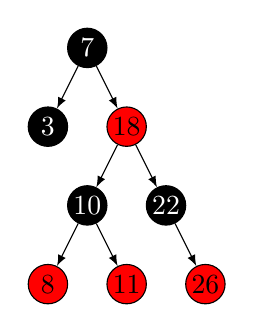
\begin{tikzpicture}[level distance=1cm, sibling distance=1cm,
    every node/.style={circle, draw, minimum size=0.5cm, inner sep=0pt},
    edge from parent/.style={draw, -latex}]
    
    % Root node
    \node[fill=black, text=white] {7}
        % Left subtree
        child {node[fill=black, text=white] {3}
            child[missing]
            child[missing]
        }
        % Right subtree
        child {node[fill=red, text=black] {18}
            child {node[fill=black, text=white] {10}
                child {node[fill=red, text=black] {8}}
                child {node[fill=red, text=black] {11}}
            }
            child {node[fill=black, text=white] {22}
                child[missing]
                child {node[fill=red, text=black] {26}}
            }
        };
\end{tikzpicture}
\end{center}
Programując - ostatni liść - $nil$ nie ma klucza, kolor jest czarny, a wskaźnik na ojca - to każdy węzeł.
Liście drzewa RB to wszystkie $nil$-węzły.\\
\textbf{Przykład} Czarna wysokość $\text{bh}(18)=2$\\

\noindent
\textbf{Lemat} Niech $T$ będzie drzewem czerwono-czarnym o $n$-węzłach. Wtedy:
\begin{align}
    \text{wysokość}(T) \leq 2\log_2(n+1)
\end{align}

\noindent
\textbf{Dowód} Czarni rodzice wchłaniają czerwone dzieci.

\begin{center}
    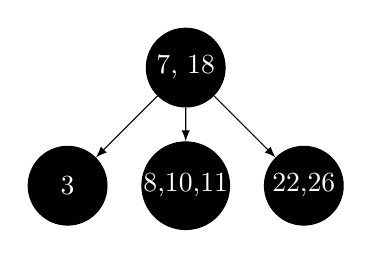
\begin{tikzpicture}[level distance=1.5cm, sibling distance=1.5cm,
        every node/.style={circle, draw, minimum size=1cm, inner sep=0pt},
        edge from parent/.style={draw, -latex}]
        
            % Root node
            \node[fill=black, text=white] {7, 18}
                % Left subtree
                child {node[fill=black, text=white] {3}}
                child {node[fill=black, text=white] {8,10,11}
                }
                child {node[fill=black, text=white] {22,26}
                };
    \end{tikzpicture}
\end{center}
W drzewie binarnym liczba liści wynosi $n+1$\\
(zawsze dokładamy 2 liście do każdego węzła - można to pokazać indukcyjnie)\\

\noindent
\textbf{2-3-4}-Tree. Liczba liści nie zmienia się.

\noindent
Mamy $n+1$ liści w drzewie czerwono-czarnym oraz w 2-3-4-drzewie (dowód - indukcyjnie)
\begin{itemize}
    \item Niech $h$ - wysokość drzewa czerwono-czarnego.
    \item Niech $h'$ - wysokość odpowiadającego mu 2-3-4-drzewa.
\end{itemize}
Zauważmy, że $h' = \text{bh}(\text{korzenia RB drzewa})$. Ograniczmy liczbę liści za pomocą funkcji od tej wysokości
\begin{align}
    2^{h'} \leq \# \text{liści} \leq 4^{h'}
\end{align}
Węzły binarne o wysokości $h'$ dają $2^{h'}$ węzłów.\\
Węzły 2-3-4 o wysokości $h'$ dają $4^{h'}$ węzłów.\\
Naszych liści jest $n+1$, zatem:
\begin{align}
    2^{h'} &\leq n+1\\
    h' &\leq \log_2(n+1)
\end{align}
Z konstrukcji wchłaniania wiemy, że $h \leq 2h'$ (ponieważ każdy czarny węzeł może wchłaniać czerwone dzieci - z 2 razy wyższego drzewa). Zatem:
\begin{align}
    h &\leq 2 \log_2(n+1)
\end{align}
\textit{W Javie 8 HashMapy były implementowane jako drzewa czerwono-czarne.}\\

\noindent
Modyfikacja drzewa czerwono-czarnego obejmuje operacje różne od BST.
Drzewo będzie wtedy zmieniać swoją strukturę aby zachować czarną wysokość - stąd również nazwa - self-balancing trees.
Operacje niemodifikujące drzewa czerwono-czarnego są tożsame z operacjami na drzewach BST.

\subsection{Insert w Red Black Trees}

RB\_Insert(T,z)
\begin{enumerate}
    \item Wstawiamy węzeł $z$ do drzewa $T$ tak jak w przypadku BST
    \item Ustawiamy kolor węzła $z$ na czerwony
    \item Naprawiamy drzewo $T$ - wywołujemy funkcję RB\_Fixup(T,z)
\end{enumerate}

Chcemy umieścić nowy węzeł ($15$) w drzewie czerwono-czarnym.
\begin{center}
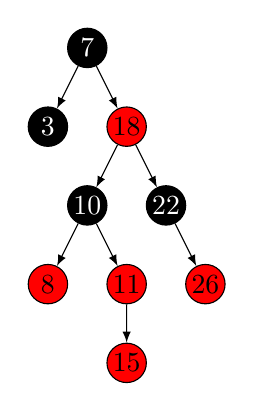
\begin{tikzpicture}[level distance=1cm, sibling distance=1cm,
    every node/.style={circle, draw, minimum size=0.5cm, inner sep=0pt},
    edge from parent/.style={draw, -latex}]
    
    % Root node
    \node[fill=black, text=white] {7}
        % Left subtree
        child {node[fill=black, text=white] {3}
            child[missing]
            child[missing]
        }
        % Right subtree
        child {node[fill=red, text=black] {18}
            child {node[fill=black, text=white] {10}
                child {node[fill=red, text=black] {8}}
                child {node[fill=red, text=black] {11}
                child {node[fill=red, text=black] {15}}
                }
            }
            child {node[fill=black, text=white] {22}
                child[missing]
                child {node[fill=red, text=black] {26}}
            }
        };
\end{tikzpicture}
\end{center}

Operacje używane w procedurze Fixup
\begin{enumerate}
    \item \texttt{recolor} - $O(1)$ - zmiana koloru węzła - z czerwonego na czarny, z czarnego na czerwony
    \item \texttt{rotate} - $O(1)$ - rotacja węzła $x$ w lewo lub w prawo.
\end{enumerate}

\begin{center}
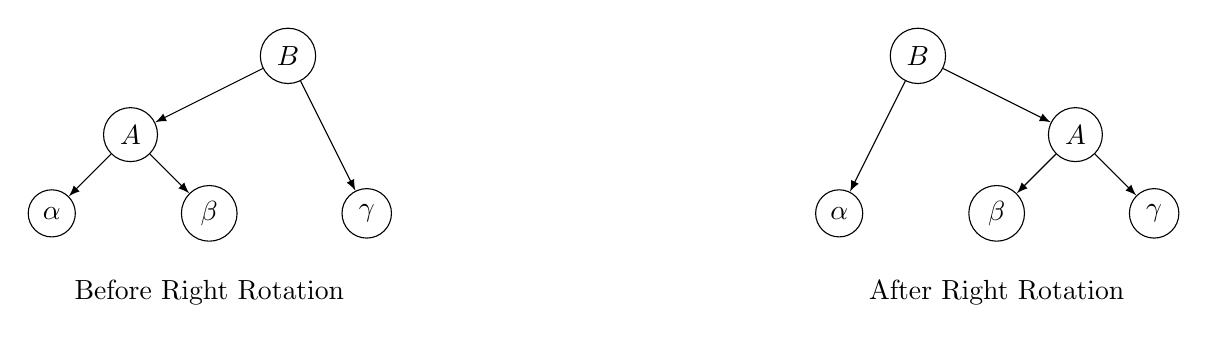
\begin{tikzpicture}
    \begin{scope}[xshift=-6cm]
        \node[draw, circle] (x) at (0, 0) {$A$};
        \node[draw, circle] (y) at (2, 1) {$B$};
        \node[draw, circle] (T2) at (1, -1) {$\beta$};
        \node[draw, circle] (T1) at (-1, -1) {$\alpha$};
        \node[draw, circle] (T3) at (3, -1) {$\gamma$};

        \draw[-latex] (x) -- (T1);
        \draw[-latex] (x) -- (T2);
        \draw[-latex] (y) -- (x);
        \draw[-latex] (y) -- (T3);

        \node at (1, -2) {Before Right Rotation};
    \end{scope}

    \begin{scope}[xshift=6cm]
        \node[draw, circle] (x) at (0, 0) {$A$};
        \node[draw, circle] (y) at (-2, 1) {$B$};
        \node[draw, circle] (T2) at (1, -1) {$\gamma$};
        \node[draw, circle] (T1) at (-1, -1) {$\beta$};
        \node[draw, circle] (T3) at (-3, -1) {$\alpha$};

        \draw[-latex] (x) -- (T1);
        \draw[-latex] (x) -- (T2);
        \draw[-latex] (y) -- (x);
        \draw[-latex] (y) -- (T3);

        \node at (-1, -2) {After Right Rotation};
    \end{scope}
\end{tikzpicture}
\end{center}

\begin{align}
    \left(\forall a\in\alpha b\in\beta c\in\gamma\right) \left(a\leq B\leq b leq A\leq c\right)
\end{align}

RB\_Fixup(T,z)

\noindent
\textbf{Case 1} - $z$ jest czerwony, ojciec $x$, wujek $w=z.p.p \leadsto \text{inne dziecko}$, $x=z.p$ jest czerwony oraz $w$-czerwony.

\begin{center}
    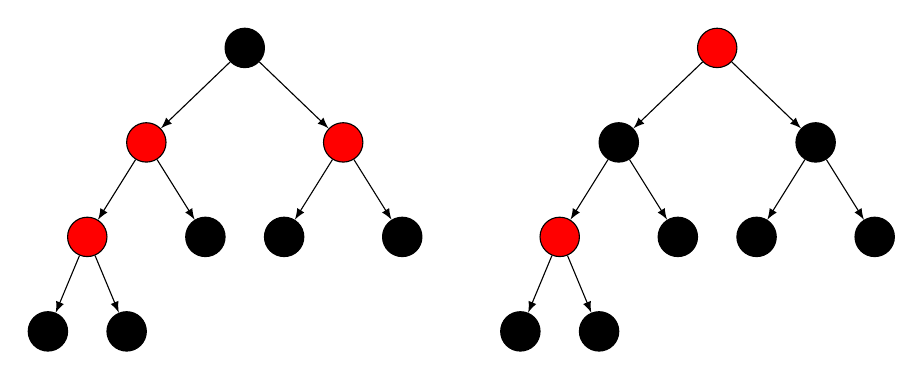
\begin{tikzpicture}[
        level distance=1.2cm, sibling distance=2.5cm,
        every node/.style={circle, draw, minimum size=0.5cm, inner sep=0pt},
        edge from parent/.style={draw, -latex},
        level 2/.style={sibling distance=1.5cm},
        level 3/.style={sibling distance=1cm}
        ]

        \begin{scope}[xshift=-3cm]
        \node[fill=black, text=white] {}
            child {node[fill=red, text=white] {}
                child {node[fill=red] {}
                    child {node[fill=black] {}}
                    child {node[fill=black] {}}
                }
                child {node[fill=black] {}}
            }
            child {node[fill=red, text=black] {}
                child {node[fill=black, text=black] {}}
                child {node[fill=black, text=black] {}}
            };
        \end{scope}

        \begin{scope}[xshift=3cm]
        \node[fill=red] {}
            child {node[fill=black] {}
                child {node[fill=red] {}
                    child {node[fill=black] {}}
                    child {node[fill=black] {}}
                }
                child {node[fill=black] {}}
            }
            child {node[fill=black] {}
                child {node[fill=black, text=black] {}}
                child {node[fill=black, text=black] {}}
            };  
        \end{scope}
    \end{tikzpicture}
\end{center}
\textbf{Case 2} - $z$ - czerwony, $x$ - czarny, $w$ - czarny, zachodzi zig-zag

\noindent
\textbf{Case 3} - $z$ - czerwony, $x$ - czarny, $w$ - czarny, bez zig-zag\\

\noindent
\textit{Poddałem się z rysowaniem tego w tikz}\\

Ostatecznie
\begin{center}
    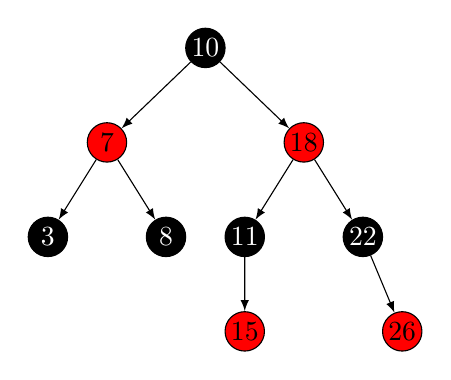
\begin{tikzpicture}[
        level distance=1.2cm, sibling distance=2.5cm,
        every node/.style={circle, draw, minimum size=0.5cm, inner sep=0pt},
        edge from parent/.style={draw, -latex},
        level 2/.style={sibling distance=1.5cm},
        level 3/.style={sibling distance=1cm}
        ]

        % Root node
        \node[fill=black, text=white] {10}
            % Left subtree
            child {node[fill=red, text=black] {7}
                child{node[fill=black, text=white] {3}}
                child{node[fill=black, text=white] {8}}
            }
            % Right subtree
            child {node[fill=red, text=black] {18}
                child {node[fill=black, text=white] {11}
                    child {node[fill=red, text=black] {15}}
                }
                child {node[fill=black, text=white] {22}
                    child[missing]
                    child {node[fill=red, text=black] {26}}
                }
            };
    \end{tikzpicture}
\end{center}

\noindent
Wnioski
\begin{itemize}
    \item Fixup - $O(\log n)$
    \item Insert - $O(\log n)$
    \item RB\_Insert - $O(\log n)$
\end{itemize}

\noindent
Inne drzewa od Red Black Trees to drzewa AVL (różnica stałych przy logarytmach), self-leaning left trees, skip list.

\textit{Następny wykład - kolejna struktura implementująca interfejs set}

\section{Lecture XI}

\subsection{Wzbogacanie struktur danych}

TBD.

\section{Lecture XII}

\subsection{Funkcje Hashujące}

Universal Hash Property. Prawdopdobieństwo kolizji dla funkcji hashującej wynosi:

\begin{align}
    Pr(h_{a,b}(x) - P_{a,b}(y)) = \frac{1}{m}
\end{align}

\begin{align}
    f_{a,b} (x) = (ax+b) \mod p\\
    g: \mathbb{Z_p} \rightarrow B \text{t.ż.} \forall_{i\in B} |\{y\in\mathbb{Z}_p : g(y) = i\}| \leq \left\lceil \frac{p}{m} \right\rceil
\end{align}
Naturalny wybór $g(y) = y \mod m$
\begin{align}
    h_{a,b}(x) = g(f_{a,b}(x))\\
    \mathcal{H} = \{h_{a,b} \text{t.ż.} a,b\in\mathbb{Z_p},\quad a\neq 0 \}
\end{align}
Lemat, Dla $x,y\in A$, t.ż. $x\neq y$ zdefiniujmy:
\begin{align}
    \delta_H (x,y) = \delta_g (\mathbb{Z}_p, \mathbb{Z}_p) = \sum_{x,yy\in\mathbb{Z}_p} \delta_g (x,y)\\
\end{align}
Funkcja $\delta$ - zliczająca kolizje.
\begin{align}
    \delta_f = \begin{cases}
        1 \quad \text{jeśli } f(x)=f(y)\\
        0 \quad \text{w p.p.}
    \end{cases}
\end{align}
Dowód. Niech $r,s\in\mathbb{Z}_p,\quad r\neq s$, para $(r,s)$ odpowiada $(f_{a,b}(x),f_{a,b}(y))$, ponieważ $a\neq 0$, $x\neq y$, $f_{a,b}(x)\neq=f_{a,b}(y)$.
Możemy skorzystać ze znajomości algebry abstrakcyjnej:
\begin{align}
    ax + b = r \mod p
    ay + b = s \mod p
\end{align}
Wiemy, że za pomocą rozszerzonego algorytmu Euklidesa możemy znaleźć unikalne $a,b$, takie że zadane kongruencje będą spełnione.
Znajdźmy takie $a,b$ ,że nie zajdzie kolizja. Zatem:
\begin{align}
    (r,s) = (f_{a,b}(x),f_{a,b}(y)), \text{to}\\
    H(a,b)(x) = H(a,b)(y) \iff g(r)=g(s), \text{stąd}\\
    \delta_H(x,y) = \sum_{x,y\in\mathbb{Z}_p} \delta_g (x,y)
\end{align}
Lemat 2. $\forall_{x,y\in A} \delta_{H}(x,y) \leq \frac{|H|}{|B|} = \frac{|H|}{m}$. Dowód:
\begin{align}
    m_i = |\{y\in\mathbb{Z}_p : g(y) = i\}| < \left\lceil \frac{p}{m} \right\rceil\\
    p, m \in \mathbb{Z} : \left\lceil \frac{p}{m} \right\rceil \leq \left(\frac{p-1}{m}\right) + 1
\end{align}
Dla ustalonego $r\in\mathbb{Z}_p$ mamy co najwyżej $\frac{p-1}{m}$ 's'-ów kolidujących. Możliwe $r\in\mathbb{Z}_p$ jest $p$ stąd mamy:
\begin{align}
    \delta_H(x,y) \leq \frac{p(p-1)}{m} = \frac{|H|}{m} = \frac{|H|}{|B|}
\end{align}
Wybierające jedną z tych funkcji ($1$ out of $m$) $\leq \frac{1}{m}$

\section{Lecture XIII}

\subsection{Programowanie Dynamiczne - Wstęp}

\textit{Dzisiejszy wykład prowadzi p. Gębala. 05.05.2024}

Dzielimy problem rekurencyjnie - ale nie rozwiązujemy go w ten sposób,
ponieważ mniejsze podproblemy nie są rozłączne - tak jak w divide and conquer.\\

\subsection{Przykład programowania dynamicznego - Ciąg Fibonacciego}

\begin{align}
    F(n) &= F(n-1) + F(n-2)\\
    F(0) &= 0\\
    F(1) &= 1
\end{align}

\subsection{Najdłuższy rosnący podciąg}

\begin{verbatim}
Input: a_1, ... a_n \in N
Ouptut: największe k, takie że istnieje:
- ciąg indeksów 1 <= i_1 < i_2 < ... < i_k <= n
- a_{i_1} < a_{i_2} < ... < a_{i_k}
\end{verbatim}

Patrzymy zakładając że znamy rozwiązanie dla $N-1$, co jeśli dodamy $n$-ty element.

\begin{enumerate}
    \item $L(i)$ - długość najdłuższego podciągu w zbiorze $[1...i]$ z elementem końcowym w $i$
    \item $L(i) = 1 + \max_{1\leq j < i} \left\{L(j) : a_i > a_j\right\}$
\end{enumerate}
Przykład
\begin{verbatim}
i    0 1 2 3 4 5
a_i  2 3 1 5 4 3
L(i) 1 2 1 3 3 2

for i=1 to n do
    L(i) = 1 + max_{1\leq j < i} {L(j) : a_i > a_j}

return max_{1\leq i \leq n} L(i)
\end{verbatim}
Programowanie dynamiczne zakłada zapisywanie poprzednich kroków, tu:
\begin{align}
    L(i) \left(\forall i\leq n\right)
\end{align}
chcąc odzyskać ciąg powinniśmy zdefiniować:
\begin{verbatim}
    prev(i) = j
\end{verbatim}

\begin{enumerate}
    \item Złożoność czasowa $O(n^2)$ (for + max)
    \item Złożoność pamięciowa $O(n)$ (każdy $L(i) 1\leq i< n$)
\end{enumerate}

\subsection{Problem wyznaczania reszty}

\begin{verbatim}
Input: 
- c_1 < c_2 < ... < c_n - zbiór nominałów \in N
- R - reszta do wydania
Output:
- minimalne k, takie że k-monet wystarczy do wydania R
\end{verbatim}
Taktyka zachłanna nie działa dla np. 1,4,5,8:
\begin{verbatim}
- zachłanny - 5,1,1,1 - 4 monety
- optymalny - 4,4 - 2 monety
\end{verbatim}
Rozwiążmy za pomocą programowania dynamicznego.
\begin{align}
    L(i) - \text{minimalna liczba monet do wydania reszty} i\\
    L(i) = 1 + \min_{1\leq j \leq n} \{L(i-c_j) : c_j \leq c_i\}\\
    L(0) = 0
\end{align}

\begin{verbatim}
c_1,c_2,c_3 = 1,4,5
Per i sprawdzamy każdą resztę 1,4,5

i    0 1 2 3 4 5 6 7 8
L(i) 0 1 2 3 1 1 2 3 2
\end{verbatim}
Złożność $O(n\cdot R)$, liczymy minimum w pętli for.
Prev backtrace
\begin{verbatim}
0 1 1 1 4 5 5 1 4
-------->
        -------->

i-4 = 4 jmp to 4
\end{verbatim}
Co jeśli mamy $\{2,4,5\}\in C$, wtedy:
\begin{verbatim}
   i 0 1
   L(i) 0 +infty
\end{verbatim}
Nie da się wydać reszty 1.\\
Fakt 1. Jeżeli zbiór monet zawiera nominał $1$, to rozwiązanie istnieje dla każdego $R\in\mathbb{N}$.
Decyzja kiedy występuje największa liczba, której nie potrafimy wydać jest problemem NP-trudnym.

Zachłanny algorytm działa dla zbioru monet, które są wielokrotnościami siebie, a w szczególności gdy
\begin{align}
\forall_{i,j} i<j \rightarrow 2c_1 \leq c_j
\end{align}

Długość danych $n\cdot \log c_n + \log_2 R = m$ - bitowe wejście, jeśli $n\log c_n \leq \log R$, wtedy:
\begin{align}
    O(nR) = O(n\cdot 2^{O(m)})
\end{align}
$R$ - liczba, a nie wielkość zapisu danych.

\subsection{Rozkład liczby pierwszej}
\begin{verbatim}
Input: p - liczba, długość log_2(p) (bitowa)
Output: Czynniki pierwsze rozkładu p
\end{verbatim}
\begin{align}
    O(\sqrt{p}) \rightarrow O(\sqrt(\sqrt{2^{\log_2(p)}})) 
\end{align}

\subsection{Knapsack - Problem Plecakowy}
\begin{verbatim}
Input:
- n par (waga, wartość) (w_i, v_i)
- ograniczenie górne na pojemność plecaka W.
Output:
- I\subseteq {1,...,n} tż:
    1. \sum_{i\in I} w_i \leq W
    2. \sum_{i\in I} v_i jest największa
\end{verbatim}
Istotnym założeniem, które musimy podjąć jest:
\begin{align}
    \forall_i w_i \leq W
\end{align}
Ponieważ musimy ignorować pojedyncze przedmioty, które są większe od pojemności plecaka.\\

\noindent
Niech $V(n)$ - maksymalna wartość na $n$ przedmiotach.
\begin{align}
    V(n,w) = \max \{v(n-1,w), V(n-1,w-w_n) + v_n \}
\end{align}
Wyjaśnienie wyboru parametrów funkcji max:
\begin{itemize}
    \item $v(n-1,w)$ - nie bierzemy $n$-tego przedmiotu
    \item $V(n-1,w-w_n) + v_n$ - bierzemy $n$-ty przedmiot, ale musimy zmniejszyć pojemność plecaka o wagę $w_n$.
\end{itemize}
Podejmijmy kroki początkowe w rekurencji:
\begin{align}
    V(0,*) &= 0\\
    V(n,W) &= \max \{V(i-1,w), V(i-1,w-w_i) + v_i\}\\
    V(0,w) &= V(j,0) = 0 \left(\forall j\in\{0,\dots,n\} i w\in{0,\dots,w}\right)
\end{align}
\begin{verbatim}
for i <- 1 to n do
    for w <- to w do
        if w_i > w then V(i,w) = V(i,w) <- V(i-1, w)
        else V(i,w) <- max(V(i-1,w), V(i-1,w-w_i) + v_i)
\end{verbatim}
\begin{align}
    O(n\cdot W)\\
    O(n\cdot 2^{O(m)})
\end{align}
Zobaczmy, że jeśli $w \leftarrow 2^{20}\cdot w$ (dodajemy 20 zer binarnie) $2^{20}$ większy czas, to jest algorytm wykładniczy.
Jeśli $W=O(n)$ to algorytm jest $n^2$.

\begin{itemize}
    \item Insertion sort - dynamicznie dodajemy element $n+1$ do posortowanej listy długości $n$
\end{itemize}

\subsection{Optymalne Mnożenie Macierzy}

\begin{verbatim}
Input: Macierze A_1,...,A_n, A_i : m_{i-1} \times m_i
Przykład (10,2) * (2,10) * (10,3)
- (10*2*10) + (10*10*3) = 500 mnożeń
- (10*2*3) + (2*10*3) = 120 mnożeń
\end{verbatim}

\begin{align}
    c(i,j) &- \text{ optymalny koszt przemnożenia } A_i \times \dots \times A_j\\
    c(i,i) &= 0\\
    c(i,j) &= \min_{i\leq k < j} \left(c(i,k) + c(k+1,j) + m_{i-1}\cdot m_k\cdot m_j \right)\\
    i<j & \text{ ostatnie mnożenie } k 
\end{align}
$\frac{n^2}{2} \text{wartość} \cdot n = O(n^3)$

Wzór rekurencyjny, ale liczymy od dołu. Należy udowodnić poprawność rozwiązania.

\section{Lecture XIV}

\subsection{Programowanie Dynamiczne - Kontynuacja}

\subsection{Grafy Skierowane}

$G=(V,E), |V|=n, |E|=m$, $V$ - wierzchołki, $E$ - krawędzie.\\

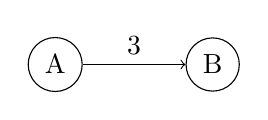
\begin{tikzpicture}
    % Nodes
    \node[circle, draw] (A) at (0, 0) {A};
    \node[circle, draw] (B) at (2, 0) {B};
    
    % Arrow with label
    \draw[->] (A) -- (B) node[midway, above] {3};
\end{tikzpicture}

\subsection{Najkrótsze ścieżki w DAG'ach - Directed Acyclic Graph}

Grafy skierowane acykliczne nie posiadają cykli. Jesteśmy w stanie posortować grafy skierowane acykliczne w kolejności topologicznej.

Graf S1. Może być więcej niż jedno źródło/ujście.

\noindent
Chcemy policzyć najkrótsze ścieżki od $S$ do każdego innego wierzchołka.

Załóżmy że chcemy dojść do $A$.

\begin{align}
    L(A) = \min\{L(S) + w(s,A), L(C) + w(C,A)\}
\end{align}

\begin{verbatim}
Input: G=(V,E)
S\in V = source vertice

for each v\in V
    L(v) = \infty // jeżeli nie ma trasy to dystans będzie ustalony na nieskończoność
L(S) = 0
for each v in V\{s} // w porządku topologicznym
    L(v) = min_((u,v)\in E) {L(u) + w(u,v)}
\end{verbatim}

Nie chcemy w programowaniu dynamicznym rekurencji, ponieważ nasze podproblemy będą się powtarzać.
To jest zasadnicza różnica między programowaniem rekurencyjnym (np. divide and conquer), a dynamicznym.
Będziemy zapamiętywać rozwiązania.

Przed pętlą mamy $\Theta(|V|)$, a w pętli $\Theta(\text{indeg}(V))$, suma wszystkich krawędzi przychodzących, czyli mamy $\Theta(|E|)$.
Złożność zadanego algorytmu to $\Theta(n+m)$, w najgorszym przypadku - mając najwięcej $m=n^2$ krawędzi, mamy $\Theta(n+n^2)$.\\

\noindent
Jak tworzyć algorytmy dynamiczne:
\begin{enumerate}
    \item Zdefinować podproblem.
    \item Zdefinować kolejność na porproblemach.
    \item Zdefiniować relację.
\end{enumerate}

\subsection{Edit Distance Problem}

Input: $w_1, w_2$ - słowa $|w_1|=n, |w_2|=m$, $\Sigma$ - alfabet
Output: $\text{EditDistance}(w_1,w_2)$ - minimalna liczba operacji dodania, usunięcia, podmiany znaków w słowach $w_1 \leadsto w_2$

\begin{verbatim}
Przykład - chcemy przejść ze SNOWY do SUNNY

S_NOWY
SUNN_Y 
010110 -> w sumie 3 operacje.
- Rozpychamy U, zmieniamy O na N, Usuwamy W. Mamy 3 operacje.

_SNOW_Y
SUN__NY
1101110 -> w sumie 5 operacji.
- Wstawiamy S, podmieniamy S na U, Usuwamy O, Usuwamy W, Wstawiamy N
\end{verbatim}

$E(i,j)$ - edit distance $w_1[1\dots i], w_2[1\dots j]$\\

Z jakich podproblemów dochodzimy do $E(i,j)$?
\begin{itemize}
    \item dodanie litery do $w_2$ - $E(i, j-1) + 1$
    \item usunięcie litery z $w_2$ - $E(i-1, j) + 1$ Dopasowujemy do $w_2$ bez jednej litery.
    \item podmiana listery z $w_2$ - $E(i-1, j-1) + 1$ Podmiana litery in place
    \item bez zmian $w_2$ - $E(i-1, j-1)$
\end{itemize}

$\text{diff}(w_1[i],w_2[i])$ - zwraca 0 lub 1 w zależnosci czy jest różnica w znakach.

\begin{verbatim}
for i=0 to m
    E(i,0) = i
for j=0...n E(0,j) = j
for i=1 to m
    for j=1 to n
        E(i,j) = min(E(i-1,j)+1, E(i,j-1)+1, E(i-1,j-1) + diff(w[i],w[j]))
\end{verbatim}

Analiza złożności obliczeniowej - pętla1 - $\Theta(m)$, pętla2 - $\Theta(n)$, pętla ostatnia $\Theta(n\cdot m)$.

Złożoność pamięciowa $\Theta(m\cdot n)$, lub jeśli nie zależy nam na krokach to $\Theta(\min\{m,n\})$
(pamiętamy każdorazowo ostatnie dwa wiersze).

\begin{verbatim}
    S N O W Y
  0 1 2 3 4 5
S 1 0 1 2 3 4
U 2 1 1 2 3 4
N 3 2 1 2 3 4
N 4 3 2 2 3 4
Y 5 4 3 3 3 3

Therefore
EditDistance("SNOWY","SUNNY") = 3
\end{verbatim}

Co na ogół jest podproblemami - np. prefix ciągu, podciąg zwarty (consecutive).

\section{Lecture XV}

\subsection{Kopiec binarny (Binary Heap)}

\begin{itemize}
    \item Pełne drzewo binarne przetrzymywane w tablicy.
\end{itemize}

\begin{verbatim}
I :  1   2   3   4  5  6  7  8  9  10
A : [16, 14, 10, 8, 7, 9, 3, 2, 4, 1]
       
        16
      /    \ 
    14      10
   /   \    / \
  8     7   9 3
 / \   /
2   4 1

left(i) = 2i (LSH)
right(i) = 2i + 1 (LSH + 1)
parent(i) = i // 2 (RSH)
size(A) = rozmiar listy
\end{verbatim}

\subsection{Własność kopca (maksymalnego)}

\begin{align}
    \forall_i A[\text{parent}(i)] > A[i]
\end{align}

\begin{itemize}
    \item Wysokość węzła to długość najdłuższej prostej ścieżki od tego węzła do liścia.
\end{itemize}

\begin{verbatim}
HEAPIFY(A, i)
    l = left(i)
    r = right(i)
    # find maximum element from i, l, r
    if (l <= size(A) AND A[l] > A[i]) 
        largest = l
    else
        largest = i
    if (r <= size(A) AND A[r] > A[largest])
        largest = r
    # end find

    # swap if so
    if largest != i
        swap(A[i], A[largest])
    HEAPIFY(A, largest)
\end{verbatim}
Przykład
\begin{verbatim}
1st step 

      16
     /    \
    i4      >10
   /  \   / \ 
  14   7 9  5
 / \   /
2   8 3

2nd step

      16
     /    \
    14      10
   /  \   / \ 
  i4   7 9  5
 / \   /
2   8 3

3rd step

      16
     /    \
    14      10
   /  \   / \ 
  8   7 9  5
 / \   /
2   i4 3
\end{verbatim}
Złożoność obliczeniowa

\begin{verbatim}
          i
     /        \
 (2/3 el.) (1/3 el.)
 ..        ..
 ..        ..
 ..  (schodek)
    
L = 2^h - 1
P = 2^{h-1} - 1 - liczba elementów
\end{verbatim}

\begin{align}
    T(n) = O(1) + T(2/3 n)
\end{align}
Z Master Theorem mamy:
\begin{align}
    a &= 1\\
    b &= \frac{3}{2}\\
    d &= 0\\
\end{align}
Zatem $\log_{\frac{3}{2}} 1 = d = 0$, więc mamy $n^d \log n = \log n$
\begin{align}
    T(n) = O(\log n)
\end{align}
\textit{floor(size(A)/2)} to indeks pierwszego nie-liścia. Pierwszym nie-liściem jest parent ostatniego liścia.
\begin{verbatim}
BuildHeap(A)
    size(A) = length(A)
    for i = floor(size(A)/2) to 1 // i--
        HEAPIFY(A,i)
\end{verbatim}

\begin{verbatim}
A: 4, 1, 3, 2, 16, 9, 10, 14, 8, 7

       4
      /  \
     1     3
   /   \  / \
  2    16 9 10
/  \  /
14 8  7

...
intermediate-steps
...

AT i = 2

       4
      /  \
     16   10
   /   \  / \
  14   7  9 3
/  \  /
2  8  1

AT i = 1 

       16
      /  \
     14   10
   /   \  / \
  8   7  9   3
/  \  /
2  4  1

RESULT: 16, 14, 10, 14, 8, 7, 9, 3, 2, 4, 1
\end{verbatim}
Złożność obliczeniowa dla BuildHeap.
\begin{align}
    |A| &= n, \frac{n}{2} \text{razy Heapify}\\
    O(n\log n)
\end{align}

\begin{fact}{Kopiec} W $n$-elementowym kopcu binarnym mamy co najwyżej $\left\lceil \frac{n}{2^{h+1}}\right\rceil$ węzłów o wysokości $h$.
Dowód.\\ Indukcja po $h$. Dla $h=0$ (liście) mamy co najwyżej $\frac{n}{2^{0+1}}$ liści to jest prawda.\\
Założenie indukcyjne $\forall_{k < h} \# \text{węzłów o wysokości} k \leq \left\lceil \frac{n}{2^{k+1}}\right\rceil$\\
Krok indukcyjny. Węzły o wysokości $k-1$ zał. ind $\leq \left\lceil \frac{n}{2^{k-1+1}}\right\rceil$.
Zatem węzłów o wysokości $h$ mamy co najwyżej $\frac{1}{2} \left\lceil \frac{n}{2^{k}}\right\rceil \leq  \left\lceil \frac{n}{2^{k+1}}\right\rceil$
\end{fact}
Złożoność obliczeniową BuildHeap można również wyrazić jako
\begin{align}
    &O\left(\sum_{h=1}^{\log n} \text{\# węzłów o wysokości h} \cdot h\right)\leq\\
    &\leq O\left(\sum_{h=0}^{\log n} \frac{n}{2^{h+1}} \cdot h\right)=\\
    &=O\left(n \sum_{h=0}^{\log n} \frac{h}{2^{h-1}}\right)=\\
    &=O\left(\frac{n}{\left(1-\frac{1}{2}\right)^2}\right)=\\
    &=O\left(n \right)
\end{align}
Istnieje HeapSort.

\subsection{Kolejka Priorytetowa (PQ)}

\begin{itemize}
    \item Insert(Q,x)
    \item Maximum(Q) : return Q[1], O(1)
    \item ExtractMax(Q) - zwraca element o najw. priorytecie, usuń z Q
    \item Increase/Decrease Key(Q,x,y) - zmieniamy z x na y
    \item Delete(Q,i)
    \item Union(Q1,Q2) : BuildHeap([Q1,Q2]), O(|Q1|+|Q2|)
\end{itemize}

\begin{verbatim}
Delete(Q, i)
    Q[i] = Q[size(Q)]
    size(Q)--
    if (Q[i] < Q[parent(i)])
        Heapify(Q, i)
    else
        while (r > 1 && Q[parent(i)] < Q[i])
            swap(Q[i], Q[parent(i)])
            i = parent(i) : O(log n)
\end{verbatim}

\begin{verbatim}
Insert(Q, key)
    size(Q)++
    i = size(Q)
    while(i > 1 && Q[parent(i)] < key)
        Q[i] = Q[parent(i)]
        i = parent(i)
    Q[i] = key : O(log n)
\end{verbatim}

\begin{verbatim}
ExtractMax(Q)
    if Q.size < 1 return null
    else
        max=Q[1]
        Q[1] = Q[size(Q)]
        size(Q)--
        Heapify(Q,1)
        return max
\end{verbatim}

\section{Lecture XVI}

\subsection{Kolejka priorytetowa - Priority Queue}

\newpage

\begin{verbatim}
Decrease/Increase Key(Q, i, newKey)
    if Q[i] > newKey # decrease
        Q[i] = newKey
        Heapify(Q, i)
    else if Q[i] < newKey # increase
        while i > 1 && Q[parent(i)] < newKey
            Q[i] = Q[parent(i)]
        Q[i] = newKey
\end{verbatim}

\begin{center}
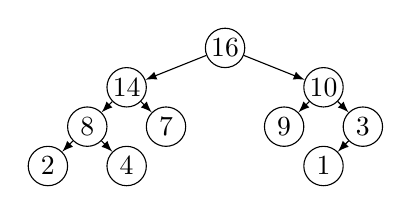
\begin{tikzpicture}[level distance=0.5cm, sibling distance=2.5cm,
    every node/.style={circle, draw, minimum size=0.5cm, inner sep=0pt},
    edge from parent/.style={draw, -latex},
    level 2/.style={sibling distance=1cm},
    level 3/.style={sibling distance=1cm}
    ]

    % Root node
    \node {16}
        % Left subtree
        child {node {14}
            child {node {8}
                child {node {2}}
                child {node {4}}
            }
            child {node {7}}
        }
        % Right subtree
        child {node {10}
            child {node {9}}
            child {node {3}
                child {node {1}}
                child[missing]
            }
        };
\end{tikzpicture}
\end{center}

\begin{verbatim}
Decrease/IncreaseKey(Q,9,11)
\end{verbatim}

\begin{center}
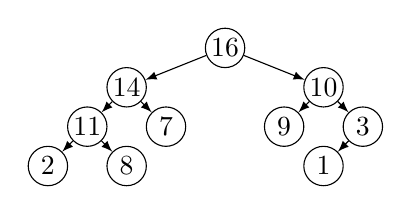
\begin{tikzpicture}[level distance=0.5cm, sibling distance=2.5cm,
    every node/.style={circle, draw, minimum size=0.5cm, inner sep=0pt},
    edge from parent/.style={draw, -latex},
    level 2/.style={sibling distance=1cm},
    level 3/.style={sibling distance=1cm}
    ]

    % Root node
    \node {16}
        % Left subtree
        child {node {14}
            child {node {11}
                child {node {2}}
                child {node {8}}
            }
            child {node {7}}
        }
        % Right subtree
        child {node {10}
            child {node {9}}
            child {node {3}
                child {node {1}}
                child[missing]
            }
        };
\end{tikzpicture}
\end{center}

% \begin{table}[h!]
% \centering
% \begin{tabular}{|l|l|l|l|}
% \hline
% \textbf{Procedura} & \textbf{Kopiec Binarny} & \textbf{Kopiec Dwumianowy} & \textbf{Kopiec Fibonacciego (Amortyzowana)}\\ \hline
% Insert & $O(\log n)$ & $O(\log n)$ & $O(1)$ \\ \hline
% Maximum & $O(1)$ & $O(\log n)$ & $O(1)$ \\ \hline
% ExtractMax & $O(\log n)$ & $O(\log n)$ & $O(\log n)$ \\ \hline
% D\/IKey & $O(\log n)$ & $O(\log n)$ & $O(1)$ \\ \hline
% Delete & $O(\log n)$ & $O(\log n)$ & $O(\log n)$ \\ \hline
% Union & $O(n_1 + n_2)$ & $O(\log (n_1 + n_2))$ & $O(1)$ \\ \hline
% \end{tabular}
% \caption{Złożoności operacji w kopcach}
% \end{table}

\subsection{Inne struktury danych}

\begin{enumerate}
    \item TREAP (1996) - Drzewo BST i Kopiec
    \item ZIP-TREE (2021)
\end{enumerate}

\subsection{Grafy}

Graf prosty to struktura $G=(V,E)$, gdzie:
\begin{itemize}
    \item $V$ - zbiór wierzchołków $\{1,\dots,n\}$, $|V|=n$
    \item $E\subseteq\{\{i,j\}:i,j\in V, i\neq j\}$, $|E|=m$
\end{itemize}

\noindent   
Graf skierowany to struktura $G=(V,E)$, gdzie:
\begin{itemize}
    \item $V$ - zbiór wierzchołków $\{1,\dots,n\}$, $|V|=n$
    \item $E\subseteq\{(i,j):i,j\in V, i\neq j\}$, $|E|=m$
\end{itemize}

\subsection{Listy sąsiedztwa}

Grafy mogą być przechowywane w postaci \textbf{Listy sąsiedztwa}. 
Używa się jej w przypadku grafów rzadkich, czyli takich które mają mało krawędzi.
Dla każdego wierzchołka $V_i$ przechowujemy listę sąsiadów.
\begin{verbatim}
V1 | 3 6
V2 | 1 3 5
V3 | 2
V4 | 1 5
V5 | 3
V6 | 
\end{verbatim}
Odpowiada następującemu grafowi:
\begin{center}
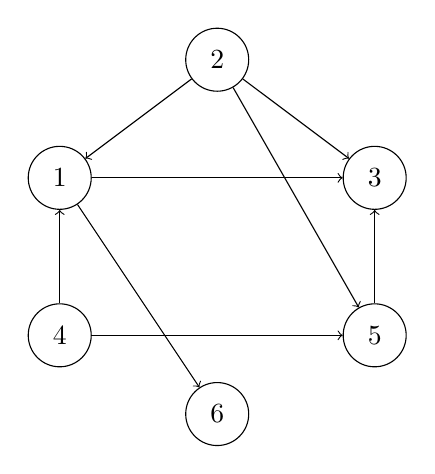
\begin{tikzpicture}[every node/.style={circle, draw, minimum size=0.8cm}, node distance=2cm]
    \node (V1) at (0,2) {1};
    \node (V2) at (2,3.5) {2};
    \node (V3) at (4,2) {3};
    \node (V4) at (0,0) {4};
    \node (V5) at (4,0) {5};
    \node (V6) at (2,-1) {6};

    \draw[->] (V1) -- (V3);
    \draw[->] (V1) -- (V6);
    \draw[->] (V2) -- (V1);
    \draw[->] (V2) -- (V3);
    \draw[->] (V2) -- (V5);
    \draw[->] (V4) -- (V1);
    \draw[->] (V4) -- (V5);
    \draw[->] (V5) -- (V3);
\end{tikzpicture}
\end{center}
\noindent
Złożoność pamięciowa przechowywania tego grafu to $O(n+m)=O(|V|+|E|)$, gdzie $m$ to liczba krawędzi.
\textbf{Wielkość grafu} definujemy przez $|V|+|E|$. Zatem jest to liniowe, względem wielkości grafu.
Sprawdzenie czy krawędź istnieje można zrobić w $O(n)$, ponieważ musimy przejść przez wszystkie sąsiadujące wierzchołki.

Można listę wzkaźnikową zastąpić drzewem BST.

\subsection{Macierz sąsiedztwa}

Niech $A=(a_{i,j}), i,j\in\{1,\dots,n\}$ będzie macierzą sąsiedztwa grafu $G=(V,E)$.
\begin{align}
    a_{i,j} = \begin{cases}
        1 & \text{jeżeli } (i,j)\in E\\
        0 & \text{jeżeli } (i,j)\notin E
    \end{cases}
\end{align}
Złożność pamięciowa to $O(n^2)$, ponieważ mamy $n^2$ elementów w macierzy. Gdy graf jest gęsty $|E| = O(n^2)$ ma to sens.
Sprawdzenie czy krawędź istnieje jest w $O(1)$, ponieważ wystarczy zbadać wartość $a_{i,j}$.\\

\noindent
;-; (Michał tu był)\\

\noindent
\textbf{Drzewo} to jest graf, który nie ma cykli.

\begin{verbatim}
EXPLORE(G,v) # G - Graf, v - wierzchołek startowy
    visited(v) = true
    previsit(v)
    for each edge (v,u) in E
        if not visited(u) EXPLORE(G,u)
    postvisit(v)
\end{verbatim}

\noindent
Mówimy, że $G$ jest \textbf{Grafem spójnym}, jeżeli dla każdego wierzchołka $v\in V$ istnieje ścieżka z $v$ do $u$.

\subsection{DFS - Depth First Search}

\begin{verbatim}
DFS(G)
    for each vertex v in G
        visited(v) = false
    for each vertex v in G
        if not visited(v) EXPLORE(G,v)
\end{verbatim}
Złożoność obliczeniowa DFS to $O(|V|+|E|)$, ponieważ w najgorszym przypadku przechodzimy przez wszystkie wierzchołki i krawędzie.
DFS działa w czasie liniowym od wielości grafu.

\subsection{Zliczanie komponentów spójnych}

\begin{verbatim}
ConnectedComponents
    cc = 1
    previsit(v):
        ccnum[v] = cc
    for each vertex v in G
        visited(v) = false
    for each vertex v in G
        if not visited(v)  
            EXPLORE(G,v)
            c++
\end{verbatim}

\subsection{Globalny zegar}

\begin{verbatim}
previsit(v):
    pre[v] = clock
    clock+=1

postvisit(v):
    post[v] = clock
    clock+=1
\end{verbatim}

\section{Lecture XVII}

\subsection{Drzewo przejścia w DFS}

Własność 1. Jeżeli istnieje ścieżka z $v$ do $u$. $u,v \in V$
\begin{itemize}
    \item $\text{pre}(v) < \text{pre}(u) < \text{post}(u) < \text{post}(v)$, jeżeli istnieje ścieżka z $v$ do $u$.
    \item $\text{pre}(v) < \text{post}(v) < \text{pre}(u) < \text{post}(u)$, jeżeli nie istnieje ścieżka z $v$ do $u$.
\end{itemize}
Nazewnictwo:
\begin{itemize}
    \item Tree Edge - krawędź, która prowadzi do potomka w drzewie DFS.
    \item Back Edge - krawędź powrotna, czyli taka, która prowadzi do wierzchołka, który już został odwiedzony.
    \item Cross Edge - krawędź do wierzchołka, który nie jest potomkiem.
    \item Forward Edge - krawędź do potomka, który nie jest bezpośrednim dzieckiem.
\end{itemize}
Włansość 2. $(u,v)\in E$.
\begin{itemize}
    \item Tree/Forward edge. $\text{pre}(u) < \text{pre}(v) < \text{post}(v) < \text{post}(u)$
    \item Back edge. $\text{pre}(v) < \text{pre}(u) < \text{post}(u) < \text{post}(v)$
    \item Cross edge. $\text{pre}(v) < \text{post}(v) < \text{pre}(u) < \text{post}(u)$
\end{itemize}
Własność 3. W grafie skierowanym istnieje cykl iff DFS występuje Back Edge.
D-d. $v_0\rightarrow v_1 \dots v_k\rightarrow v_0$ jest cyklem.
Powiedzmy, że DFS odwiedzi jako pierwszy w tym cyklu wierzchołek $v_i$, dalej eksplorując natknie się na $v_{i-1}$,
wtedy krawędź $(v_i,v_{i-1})$ będzie Back Edge, ponieważ $v_{i-1}$ jest już odwiedzony.

\subsection{Sortowanie topologiczne}

Sortowanie topologiczne elementów grafu. Nie jesteśmy w stanie posortować grafu cyklicznego.
Chcemy sortować topologicznie grafy skierowane acykliczne (DAG).

\begin{itemize}
    \item $G=(V,E)$ - graf skierowany acykliczny.
    \item $(V,\prec)$ - porządek topologiczny na $V$.
\end{itemize}
Musimy zachować $\text{post}(u) < \text{post}(v)$, jeżeli istnieje krawędź $(u,v)\in E$.
Pomysł:
\begin{enumerate}
    \item Najpierw wykonajmy DFS zapisując wartości $\text{pre},\text{post}$
    \item Zwróćmy wierzchołki w malejącym porządku po $\text{post}$.
\end{enumerate}

\noindent
W grafie skierowanym $G=(V,E)$ powiemy, że wierzchołki $u,v\in V$ są \textbf{połączone}, jeżeli istnieje ścieżka z $u$ do $v$ oraz z $v$ do $u$.

\noindent
Definicja. Silnie spójna komponenta grafu skierowanego $G=(V,E)$.
Będziemy mówić, że $v_1, \dots, v_k$ tworzą silnie spójną kompnentę w grafie $G$, jeśli:
\begin{itemize}
    \item $\forall_{i,j} \quad v_i, v_j \in V$ są połączone.
    \item Nie istnieje wierzchołek $u\in V$ taki, że $u$ jest połączony z każdym $v_i$ i $v_j$.
\end{itemize}

\noindent
Tworzymy Metagraf Silnie spójnych składowych.
\begin{itemize}
    \item \textbf{Źródłem (Source)} jest wierzchołek, do którego nie wchodzi żadna krawędź z innej kompnenty.
    \item \textbf{Ujściem (Sink)} jest wierzchołek, z którego nie wychodzi żadna krawędź do innej kompnenty.
\end{itemize}

\noindent
Własność 4. Wierzchołek z najwyższą wartością $\text{post}$ w silnie spójnej kompnencie jest źródłem tej kompnenty.\\

\noindent
Własność 5. Niech $C, C'$ będą silnie spójnymi składowymi w grafie skierowanym $G$,
oraz istnieje w $G$ krawędź $(u,v)$, gdzie $u\in C$ i $v\in C'$. Wtedy maksymalna wartość $\text{post}$ wierzchołka z $C$ jest większa niż maksymalna wartość $\text{post}$ z $C'$.\\
D-d. Rozważmy dwa przypadki
\begin{itemize}
    \item DFS najpierw odwiedzi wierzchołek $u\in C$ przed wierzchołkami z $C'$. Jasno widzimy, że $\text{post}(u) > \text{post}(v)$.
    \item DFS najpierw odwiedzi wierzchołek z $v\in C'$ przed wierzchołkami $C$. DFS wyeksploruje wierzchołki z $C'$ oraz pozostałe silne spójne składowe dalej,
     ale explore nie przejdzie przez $C$, ponieważ nie może się cofnąć. Następne posty w $C$ będą miały zatem większą wartość niż posty w $C'$.
\end{itemize}

\noindent
Własność 6. Niech $G^R=(V,E^R) : E^R =\{(v,u), (u,v)\in E\}$. Źródło grafu $G^R$ jest ujściem w meta-grafie z $G$.

\noindent
Algorytm.
\begin{itemize}
    \item Input: $G=(V,E)$ - graf skierowany.
    \item Output: Metagraf silnie spójnych składowych $G$
\end{itemize}
Korki algorytmu:
\begin{enumerate}
    \item Wylicz $G^R$
    \item Wykonaj DFS na $G^R$ i zapisz $\text{post}$.
\end{enumerate}
\begin{verbatim}
    while G nie pusty
        v = wierzchołek z największą wartością post
        S = EXPLORE(G,v)
        V = V \ S
\end{verbatim}
Złożność obliczeniowa algorytmu to $O(|V|+|E|)$, ponieważ wyznaczamy $G^R$, wykonujemy DFS na grafie $G^R$ oraz $G$.

\section{Lecture XVIII}

Pathfinding

\section{Lecture XIX}

\subsection{Dowód dla Dijkstra Algorithm}

1. Prezentujemy założenie indukcyjne. $d\in \mathbb{R}_{+}, w \in \mathbb{R}_{+}$
\begin{align} 
    \left(\forall_{x\in\mathbb{R}}\right) \text{dist}(x) \leq d
\end{align}

\noindent
Czy możemy wagi krawędzi rozszerzyć z $\mathbb{R}_{+}$ na $\mathbb{R}$?

\begin{itemize}
    \item W grafie, w którym znajdują się ujemne cykle nie ma sensu przeprowadzać Algorytmu Dijsktry.
    \item W grafie, w którym nie znajdują się ujemne cykle można przeprowadzić Algorytm Dijkstry, pomimo występowania krawędzi o ujemnych wagach. Nie zmienia to faktu, iż dowód indukcyjny takigo algorytmu jest niemożliwy.
\end{itemize}

W algorytmie Dijkstry wykonujemy procedurę update, która jest bezpieczna na wielokrotne jej powtarzanie.
Jeśli dystans do $u$ był już ustawiony poprawnie oraz na najkrótszej ścieżce od S przechodzi przez $u$ do $v$, 
to wtedy dystans do $v$ zostanie poprawnie ustawiony, zakładąc, że dystans do $u$ jest poprawnie ustawiony.

\begin{verbatim}
update((u,v) \in E)
    if dist(u) + w(u,v) < dist(v):
        dist(v) = dist(u) + w(u,v)
        prev(v) = u
\end{verbatim}

Jaka jest możliwie najdłuższa możliwa ścieżka w grafie, którego krawędzie mogą mieć ujemne wagi.
Najdłuższa ścieżka (w sensie liczby krawędzie) będzie przechodzić przez $|V|-1$ krawędzi.
Nie może być dłuższa, ponieważ wtedy powstałaby ścieżka długości $|V|$, która musiałaby być cyklem z krawędziami ujemnej wagi, a założyliśmy że tak nie jest.

\subsection{Algorytm Bellmana-Forda}

\begin{itemize}
    \item Input: $G=(V,E), e\in E: w_e \in \mathbb{R}$, bez ujemnych cykli $s\in V$
    \item Output: $\forall v\in V$, do którego da się dojść z $S$, mamy wyznaczone $\text{dist}(v),\text{prev}(v)$ - najkrótszą możliwą ścieżkę
\end{itemize}

\begin{verbatim}
for all v in V
    dist(v) = infinity
    prev(v) = null
dist(s) = 0
repeat |V|-1 times
    for all e in E
        update(e)
\end{verbatim}

Złożoność obliczeniowa algorytmu - $O(|V|\cdot |E|)$

\subsection{Algorytmy Zachłanne}

\subsection{Definicja Drzewa}

\begin{definition}{Drzewo}
    Acykliczny spójny graf nieskierowany.
\end{definition}

\subsection{Minimalne drzewo rozpinające, MST - Minimum Spanning Tree}

Minimalne drzewo ropzinające jest potrzebne do stworzenia najtańszych ścieżek między wierzchołkami.

\begin{itemize}
    \item Input: Graf $G=(V,E), e\in E w_e$
    \item Output: Drzewo $T=(V,\mathcal{E})$ t.ż. $\mathcal{E}\subseteq E$ oraz $\text{weight}(T)=\sum_{e\in E} w(e)$ jest minimalna.
\end{itemize}

Chcielibyśmy z grafu stworzyć drzewo, o minimalnej sumie wag składających się na niego krawędzi.

Własności drzewa rozpinającego:

\subsection{Własności minimalnego drzewa rozpinającego}

\begin{itemize}
    \item Usunięcie krawędzi należącej do cyklu nie rozspójni grafu.
    \item Drzewo o $n$ wierzchołkach ma $n-1$ krawędzi.
    \item Definicja Równoważna. Każdy spójny nieskierowany graf $G=(V,E)$ taki, że $|E|=|V|-1$ jest drzewem.
    Załóżmy, że $G$ ma cykl i $e\in E$ nalezy do tego cyklu. Wtedy $G-e$ jest grafem spójnym z własności pierwszej. Ale nasz graf 
    $G$ ma $|V|-1$ krawędzi, więc nie może być spójny, ponieważ usunięcie krawędzi $e$ spowoduje rozspójnienie grafu, zatem
    $G$ nie może mieć cyklu, więc jest drzewem.
\end{itemize}

\begin{itemize}
    \item Minimalne drzewo rozpinające nie musi być unikalne.
\end{itemize}

\subsection{Cut Property}

Niech $X$ będzie podzbiorem krawędzi minimalnego drzewa rozpinającego grafu $G=(V,E)$. Wybierzmy podzbiór wierzchołków $S\subset V$,
takich, że żadna krawędź z $X$ nie przechodzi pomiędzy wierzchołkami z $S$ i $V\setminus S$. Niech $e\in E$ będzie krawędzią o najmniejszej
wadze, która przechodzi pomiędzy $S$ i $V\setminus S$. Wtedy $X\cup \{e\}$ należy do minimalnego drzewa rozpinającego grafu $G$.

\noindent 
Dowód. Niech $T$ to minimalne drzewo rozpinające grafu $G$. Z założeń wiemy, że krawędzie należące do $X$ są częścią 
minimalnego drzewa rozpinającego. Jeśli $e\in T$ to wszystko jest ok. Założmy zatem, że $e\notin T$. Wtedy zmodyfikujmy
$T$ w taki sposób, że $\widetilde{T}=T\setminus \{e'\}\cup \{e\}$, gdzie $e'$ jest krawędzią z $T$, która przechodzi pomiędzy $S$ i $V\setminus S$.
$\widetilde{T}$ jest nieskierowany, ponieważ wszystkie krawędzie biorą się z grafu nieskierowanego. Poprzez usunięcie krawędzi $e'$ krawędź $e$ jest jedyną
krawędzią, która przechodzi pomiędzy $S$ i $V\setminus S$, zatem nie może tworzyć cyklu. Spójność grafu $\widetilde{T}$ jest zachowana, ponieważ
usunięcie krawędzi $e'$ nie rozspójnia grafu. $\widetilde{T}$ ma $|V|-1$ krawędzi, zatem jest drzewem.

\noindent
Skoro $T$ jest MST:
\begin{align}
    \text{weight}(\widetilde{T}) &= \text{weight}(T) - \text{weight}(e') + \text{weight}(e) \\
    \text{weight}(T) &\leq \text{weight}(\widetilde{T}) \\
    w(e) &\leq w(e') \text{ Skoro $e$ jest krawędzią o najmniejszej wadze}
\end{align}

W takim razie $\text{weight}(\widetilde{T}) = \text{weight}(T)$, zatem $\widetilde{T}$ również jest minimalnym drzewem rozpinającym grafu $G$.
Zatem $X\cup \{e\}$ jest częścią minimalnego drzewa rozpinającego grafu $G$.

\section{Lecture XX}

\subsection{Algorytm Kruskala}

\section{Lecture XXI}

\subsection{Problem Min-Cut}

\begin{itemize}
    \item Input: Graf $G=(V,E)$.
    \item Output: Minimalny zbiór krawędzi rozspójniający graf.
\end{itemize}
Niech zbiór $A$ będzie zbiorem krawędzi łączących $S$ i $V-S$.
Możemy zbudować minimalne drzewo rozpinające, w $S$ $V-S$:
\begin{align}
    \text{Pr}(A\in\text{MinCut}) \geq \frac{1}{n(n-1)}
\end{align}
Możemy stworzyć algorytm Kruskala (nieskierowany, więc nie musimy sortować krawędzi) do ostatniego jego kroku, w którym miałby on znaleźć ostatnią
krawędź, która przechodzi pomiędzy $S$ i $V-S$. Wtedy ta krawędź rozspójniłaby graf.

Powtórzmy $\Theta(n^2)$ razy algorytm Kruskala, aby znaleźć minimalne przecięcie - wraz z $n$ dążącym do nieskończoności porafimy wyznaczyć najmniejszy zbiór rozcinający.

Złożoność całej procedury to $\Theta(n^2) \cdot O(|E|\log |V|)$.

Zapiszmy dla klaryfikacji w worst case $|E|=|V|^2$, więc $\log(|E|) = O(\log |V|^2) = O(2\log |V|) = O(\log |V|)$.

Pokażmy postulowaną wyżej nierówność. Załóżmy, że $|\text{MinCut}|=C$.
Załóżmy, że jesteśmy w kroku algorytmu Kruskala, w którym mamy $k$ komponent.
Liczba krawędzi, które możemy wybrać to będzie co najmniej $\frac{kC}{2}$
Prawdopodobieństwo, że wybierzemy krawędź z MinCuta wynosi co najmniej:
\begin{align}
    \frac{C}{\frac{kC}{2}} &= \frac{2}{k} \geq \text{Pr}(\text{że wybiorę krawędź} \in\text{MinCut})\\
    \text{Pr}(\text{że nie wybiorę krawędzi} \in \text{MinCut}) &\geq 1 - \frac{2}{k} = \frac{k-2}{k}\\
    \text{Pr}(A\in\text{MinCut}) &\geq \frac{n-2}{n} \cdot \frac{n-3}{n-1} \cdot \frac{n-4}{n-2} \cdot \dots \cdot \frac{2}{4} \cdot \frac{1}{3} = \\
    &= \frac{2}{n(n-1)}
\end{align}
Ogólny framework dający cut property.
\begin{verbatim}
x={}
repeat until |X|=|V|-1
    wybierz S \subset V, dla którego w X nie ma krawędzi pomiędzy S i V\S.
    znajdź krawędź e \in E o najmniejszej wadze pomiędzy S i V\S.
    X = X u {e}
\end{verbatim}
Kruskal nie wybiera S-explicite, ponieważ wybiera najtańszą krawędź.

\subsection{Algorytm Prima}

\begin{verbatim}
Prim(G=(V,E), (w_i)i=1,...|E|) -> MST dla grafu G
    for v in V 
        cost(v) = infinity
        prev(v) = null
    cost(u) = 0
    H = MakePQ(V) // priorytetem jest cost(v)
    while H is not empty
        v = ExtractMin(H)
        for each {v,z} in E
            if cost(z) > w(v,z)
                cost(z) = w(v,z)
                prev(z) = v
                decreaseKey(H,z)
\end{verbatim}

\subsection{Kodowanie Huffmana}

\begin{itemize}
    \item Digitalizacja analogowego dźwięku, próbkujemy np $44.1$KHz, czyli 44 tysiące próbek na sekundę.
    \item $\Gamma$ - alfabet, na który zmapujemy próbki. $\Gamma=\{A,B,C,D\}$
    \item Zmapuj elementy alfabetu na ciągi bitowe.
\end{itemize}
$50 \cdot 60 \cdot 44100 \cdot 2 \implies 260$ milionów bitów.

Jeśli częstotliwości znaków $A=70m, B=3m, C=20m, D=37m$, to ustawmy kody prefix free: $A=0,D=10,C=110,D=111$, 
wtedy: $70m \times 1 + 37m \times 2 + 20m \times 3 + 3m \times 3 = 213$ milionów bitów.

Prefix-free code możemy przedstawić za pomocą drzewa binarnego, takiego że
h
\end{document}
